\chapter{Our Work}
\label{chap:prelim-exp}

\section{Overview}
This work presents a method dealing with challenges where we have a fully annotated dataset, however, very small in size (TNBC dataset \cite{TNBC-nuclei-seg-extended}), and a large dataset but weakly annotated (TIGER dataset \cite{tiger_dataset}). We aim to overcome these challenges by implementing a hybrid approach for the semantic segmentation of lymphocyte cells. The overview of the whole approach is displayed in Figure \ref{fig:dg-overview}. The hybrid method consists of a preprocessing module, which prepares data for training and evaluation; then the pseudo-mask creating module, which creates the pseudo-masks for the TIGER dataset images. The resulting image patches are then used for the training of the deep learning segmentation model, which we describe in Section \ref{section:dl-model}.

\begin{figure}[H]
\begin{centering}
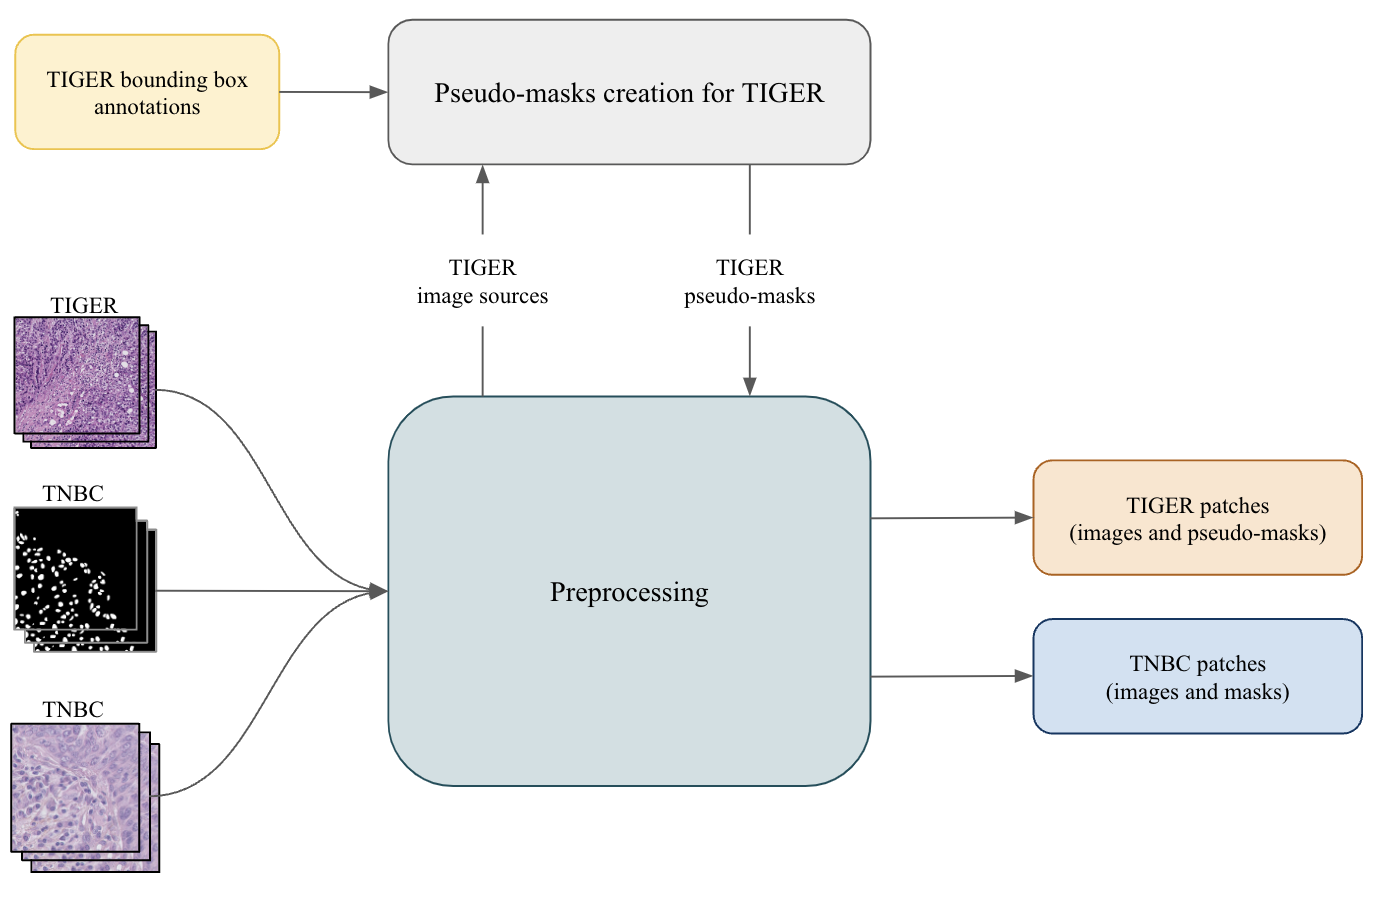
\includegraphics[width=\textwidth]{assets/images/for_presentation/dg-overview.png}
\par\end{centering}
\caption{The overview of our hybrid approach for semantic segmentation. 
\label{fig:dg-overview}}
\end{figure}

Firstly, we try to train and validate a model on the small dataset itself. Then we use preprocessing and computer vision techniques to generate various pseudo-mask sets out of bounding-box annotations for the weakly annotated dataset and train a model on it, which is again validated on the small, fully annotated dataset. Then we try to identify and select the best fusing strategy for the mask sets, to utilize different abilities of the sets to capture the cell region. Next, we select the best model (with the most successful mask-fusing strategy) and fine-tune it using a portion of the data in the fully annotated dataset. We evaluate each of these experiments with the Dice coefficient and IoU. We start with the fundamental part - the description of the datasets used.

\section{Datasets}
\label{sec:datasets}

\paragraph{TIGER} In our work, we use the Tumor Infiltrating Lymphocytes in Breast Cancer - TIGER - dataset, which was released with the challenge under the same name on the Grand Challenge platform \cite{tiger_dataset}. It contains H\&E-stained WSIs of HER2-positive and TNBC breast cancer tissues obtained by core needle biopsies or surgical resections. The images were scanned using 20x magnification. The dataset is released in three formats. We work with the one called WSIROIS. The WSIs come from three different institutions:

\begin{enumerate}
    \item TCGA (151 WSIs) dataset, which contains images of TNBC from the TCGA-BRCA archive, annotations, and magnification, was adopted to be in line with those used further.
    \item RUMC (26 WSIs) images of both TNBC and HER2-positive breast cancer obtained from Radboud University Medical Center in the Netherlands, annotated by a panel of board-certified pathologists.
    \item JB (18 WSIs) images of both TNBC and HER2-positive breast cancer obtained from Jules Bordet Institute in Belgium, annotated by a panel of board-certified pathologists.
\end{enumerate}

The RUMC and JB WSIs contain 3 annotated ROIs with a size of approximately $500\!\times\!500$ \textmu m. The WSIs obtained from TCGA are more specific. This dataset was created by merging two other datasets: the BCSS (151 WSIs) and the NuCLS (124 WSIs). The NuCLS is a subset of the BCSS dataset. In the BCSS dataset, the tissue in a single large ROI is annotated, but no cells are annotated. In the NuCLS, a variable number of smaller ROIs are selected within the large ROI (same large ROI as in the BCSS), and these are densely annotated for multiple cell types. Annotations are adapted to match the other used annotations, as was mentioned.

The WSIROIS format contains:

\begin{itemize}
    \item WSI level annotations, wherein each WSI contains manual annotations of ROIs. Different tissue types are annotated with polygons, namely: invasive tumor, tumor-associated stroma, in-situ tumor, healthy glands, necrosis not in-situ, inflamed stroma, and rest. Most ROIs have also annotated plasma cells and lymphocytes. These were annotated using point annotations and then a bounding box was constructed and centered on the point of annotation with the size of $6\!\times\!6$ \textmu m, $8\!\times\!8$ \textmu m, or $9\!\times\!9$ \textmu m. Annotations for WSIs are released in XML format and also as a multi-resolution TIF image.
    \item ROI level annotations, where authors cropped the ROIs from WSIs and stored them as PNG files. Tissue type annotations are released as PNG images, containing pixel-level masks, and cell annotations are released in the COCO format - a JSON file containing file paths (the PNG images of ROIs) with IDs and metadata and corresponding annotations of bounding box position and size.
\end{itemize}

We further work with the part of the dataset that has ROI-level annotations. This part of the dataset consists of 1,879 (1,744 from TCGA, 81 from RUMC, 54 from JB) ROIs cropped from 44 (124 from TCGA, 26 from RUMC, 18 from JB). Together, they contain 30,524 annotated cell nuclei.

An example of an image and its bounding box labels can be seen in Figure \ref{fig:tiger-with-without}.

\begin{figure}[H]
  \centering
  \begin{subfigure}[b]{0.32\textwidth}
    \centering
    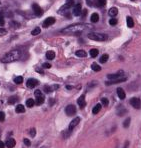
\includegraphics[width=\linewidth]{assets/images/for_presentation/image_TCGA-EW-A1P8-01Z-00-DX1.E9852193-8CDD-49EF-B49B-DA6931198F0D_[8391, 13690, 8532, 13838].png}
    \subcaption{Without annotations}\label{fig:tiger-img}
  \end{subfigure}%
  \quad
  \begin{subfigure}[b]{0.32\textwidth}
    \centering
    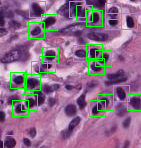
\includegraphics[width=\linewidth]{assets/images/for_presentation/bbox_TCGA-EW-A1P8-01Z-00-DX1.E9852193-8CDD-49EF-B49B-DA6931198F0D_[8391, 13690, 8532, 13838].png}
    \subcaption{With annotations}\label{fig:tiger-bbox}
  \end{subfigure}%
  \caption{Example of TIGER image without and with annotations of TILs \cite{tiger_dataset}.}
  \label{fig:tiger-with-without}
\end{figure}

\paragraph{TNBC} Triple Negative Breast Cancer Nuclei Segmentation dataset \cite{TNBC-nuclei-seg}, is an open dataset consisting of 11 patients with breast cancer, with varying numbers of images for each patient, provided regions of interest (ROIs) in PNGs. Together, it has 50 annotated ROIs of size $512\!\times\!512$, scanned with 40x magnification. Specifically, we use the extended version of this dataset \cite{TNBC-nuclei-seg-extended}, where annotations of cell classes were added. Each image has a corresponding pixel mask, where each pixel is labeled by the class it represents. There are 11 different cell classes, plus background and unknown classes. We also note that this extended version of the dataset provides images of brain tissue, but since it is not part of our work, we only work with the images of breast cancer. An example image with its ground truth mask, already relabeled so only lymphocytes are annotated, can be seen in Figure \ref{fig:tcga-with-without}.

\begin{figure}[H]
  \centering
  \begin{subfigure}[b]{0.32\textwidth}
    \centering
    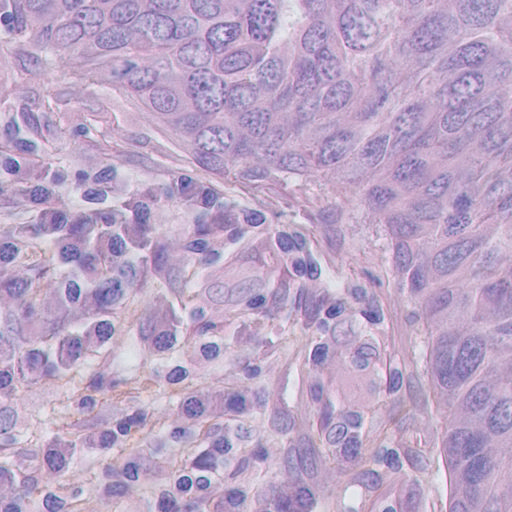
\includegraphics[width=\linewidth]{assets/images/for_presentation/image_10_1.png}
    \subcaption{Image}\label{fig:tcga-img}
  \end{subfigure}%
  \hfill
  \begin{subfigure}[b]{0.32\textwidth}
    \centering
    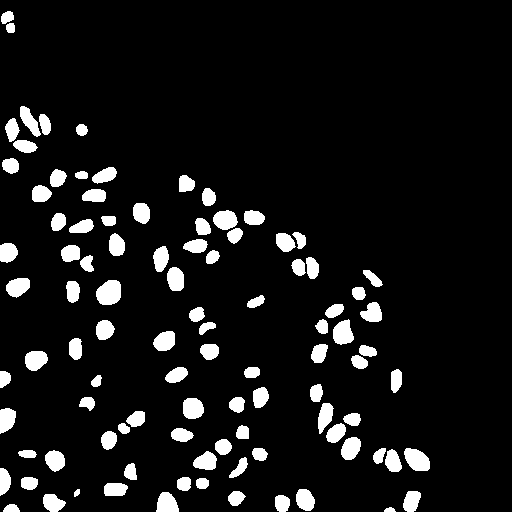
\includegraphics[width=\linewidth]{assets/images/for_presentation/mask_10_1.png}
    \subcaption{Mask}\label{fig:tcga-mask}
  \end{subfigure}%
  \hfill
  \begin{subfigure}[b]{0.32\textwidth}
    \centering
    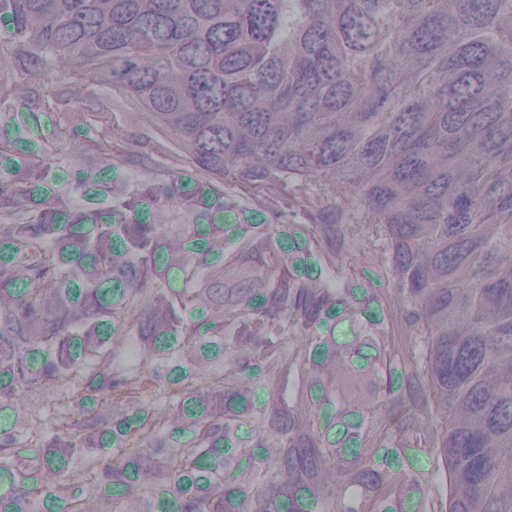
\includegraphics[width=\linewidth]{assets/images/for_presentation/overlay_10_1.png}
    \subcaption{Image with mask overlay}\label{fig:tcga-overlay}
  \end{subfigure}%
  \caption{Example of TNBC image, mask, and overlay, where TILs are annotated \cite{TNBC-nuclei-seg-extended}.}
  \label{fig:tcga-with-without}
\end{figure}

\section{Deep Learning Model}
\label{section:dl-model}

\subsection{Architecture}
As a deep learning model for semantic segmentation, we employ the U-Net architecture. U-Net is a powerful architecture, and as we mentioned in Chapter \ref{chapter:dnn}, in Section \ref{chapter:dnn-section:arch}, it is also widely used in the medical imaging domain. Specifically, we use the ResNet-34 encoder as the U-Net's backbone, which is already pretrained on the ImageNet dataset. This choice was based on the fact that residual blocks further improve the U-Net's ability to learn, as we continue to write in Section \ref{chapter:dnn-section:arch} of Chapter \ref{chapter:dnn}. In the state-of-the-art, which we present in Chapter \ref{chapter:related}, authors in \cite{Zhang2022, Liang2023} also use ResNet architectures, and specifically, ResNet-34 is used in \cite{Lin2023}. The inspiration to initialize the encoder with weights pretrained on the ImageNet dataset came from the state-of-the-art works as well, where a similar approach was used in \cite{Zhang2022, Lin2023, Liang2023}. The full architecture of the model can be seen in Figure \ref{fig:our-architecture}.

\begin{figure}[H]
\begin{centering}
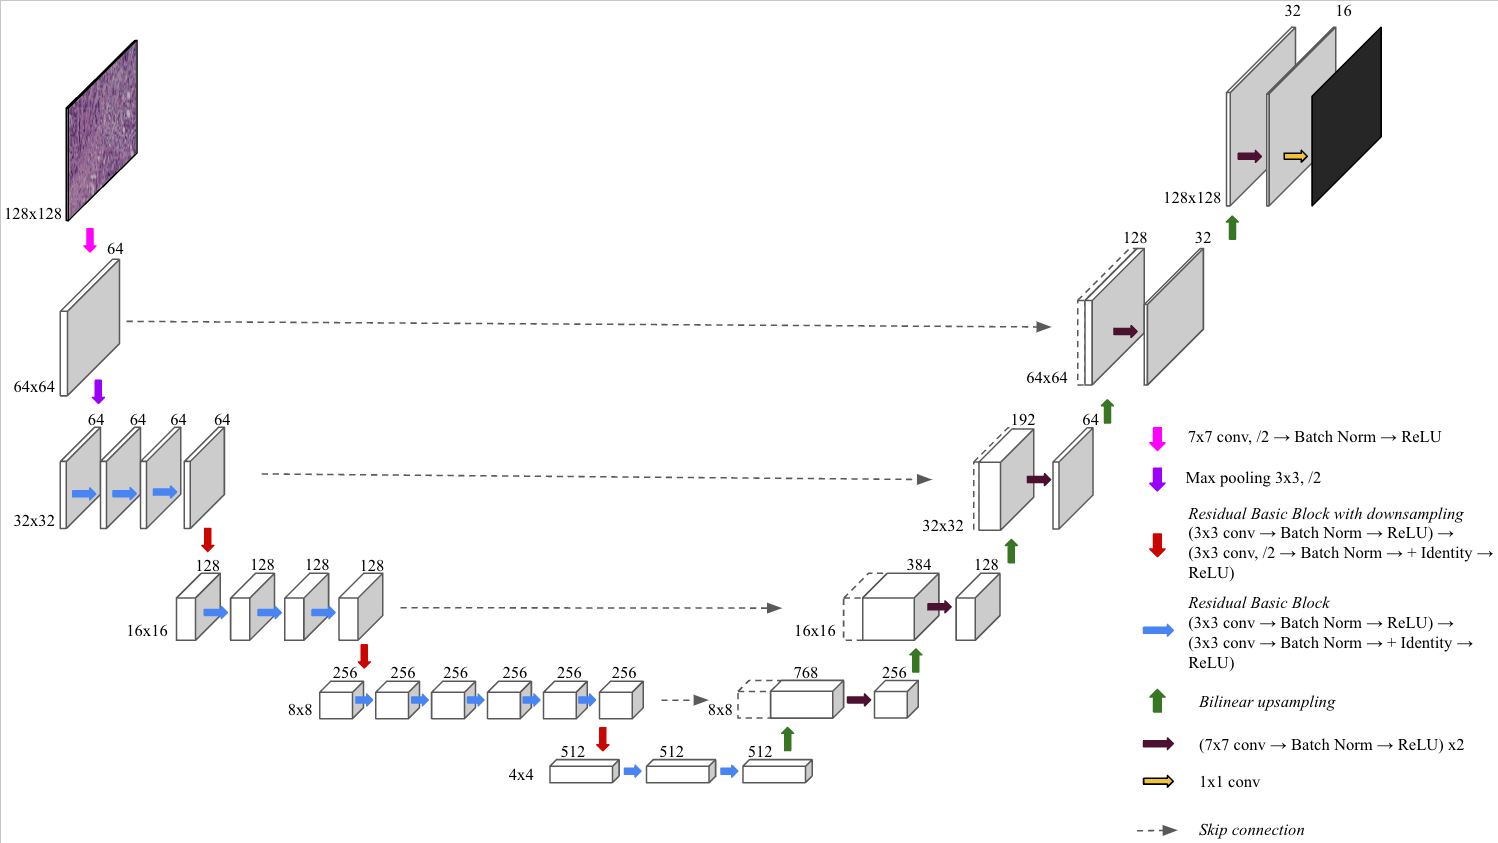
\includegraphics[width=\textwidth]{assets/images/for_presentation/our_architecture.png}
\par\end{centering}
\caption{The architecture of our model. 
\label{fig:our-architecture}}
\end{figure}

This model is being used in all our experiments as the segmentation model. The training setup and model's hyperparameters remain the same in every experiment as well. 

\subsection{Input and Output Specifications}
The input for the model is an image of size $128\!\times\!128$ pixels in a 3 - RGB - channel space. The model's segmentation head produces a binary mask of size $128\!\times\!128$ pixels and a depth of 1. The output mask is then run through the sigmoid function to squeeze the values between 0 and 1. A threshold of 0.5 is applied to this mask as pixels with a value less than 0.5 are predicted background and labeled with a number 0, and pixels with a value greater than or equal to 0.5 are predicted TILs and labeled with a number 1.

\subsection{Loss Function}
The loss function used during training is the Dice Loss function. This loss function is the preferred function to be used in the segmentation of objects and is also frequently used in the medical imaging domain, as described in \cite{Zhang2021}.

\subsection{Optimization}
We used the Adam optimizer, and the initial learning rate was set to 0.001, and it was reduced every 5 epochs by a factor of 0.1. Early stopping was also used, where the patience was set to 10 checks - if the validation loss was not improved during the training and it got worse at least on 10 checks, the training stopped to prevent overfitting. Checks were performed during every validation run, after every epoch.

\subsection{Training}
Every training was set to run for 100 epochs, but it could be stopped earlier. The batch size was set to 16 samples. Checkpoints of the model were periodically saved every epoch, always the best checkpoint (in terms of validation loss). If the CUDA framework is available, the training runs on the GPU; if not, then on the CPU. During the training stage, we monitored the model's performance on various variables. These included accuracy, recall, precision, Dice coefficient, IoU, and the running loss.

For training purposes, we further split the training data into the training subset (80\% of the whole training dataset) and the validation subset (20\% of the whole training dataset). Then, in each epoch, we let the model process the whole training subset (in the form of batches) while monitoring and logging the aforementioned variables. After each epoch, we set the model into validation mode. In this mode, the model does not update its parameters. We let it process the validation subset and also monitor and log the variables, out of which the most interesting for us is the validation loss, since this is used both for the early stopping and for saving the checkpoints. After the validation was completed, we set the model into the training mode again, where it could further update its parameters. This whole process was repeated until the training was finished, and the model could be evaluated on the testing dataset.

\section{Evaluation Methods}
Upon completing the training process, we initiated the final evaluation of the segmentation model. The best-performing model, determined by the lowest validation loss, was loaded from the saved checkpoint and set to evaluation mode to prevent any parameter updates. Subsequently, the model processed the entire testing dataset, and the final testing metrics were computed.

We assessed the model using both quantitative and qualitative methods. The quantitative evaluation included the Dice coefficient and IoU metrics - we describe these in more detail and why they are most suitable for segmentation tasks in Chapter \ref{chapter:dnn}, in Section \ref{chapter:dnn:eval}. For qualitative assessment, we visualized the predicted binary masks alongside the ground truth masks to facilitate direct comparison.

\section{Data Preprocessing}
Since we work with two very distinct datasets, and furthermore, the TIGER dataset is composed of three other datasets, we need to employ a robust preprocessing framework to align all datasets on the same level. In Figure \ref{fig:dg-preprocessing}, we can see how the images and masks from each dataset are preprocessed. Below, we describe each preprocessing step for each image and mask set.

\begin{figure}[H]
\begin{centering}
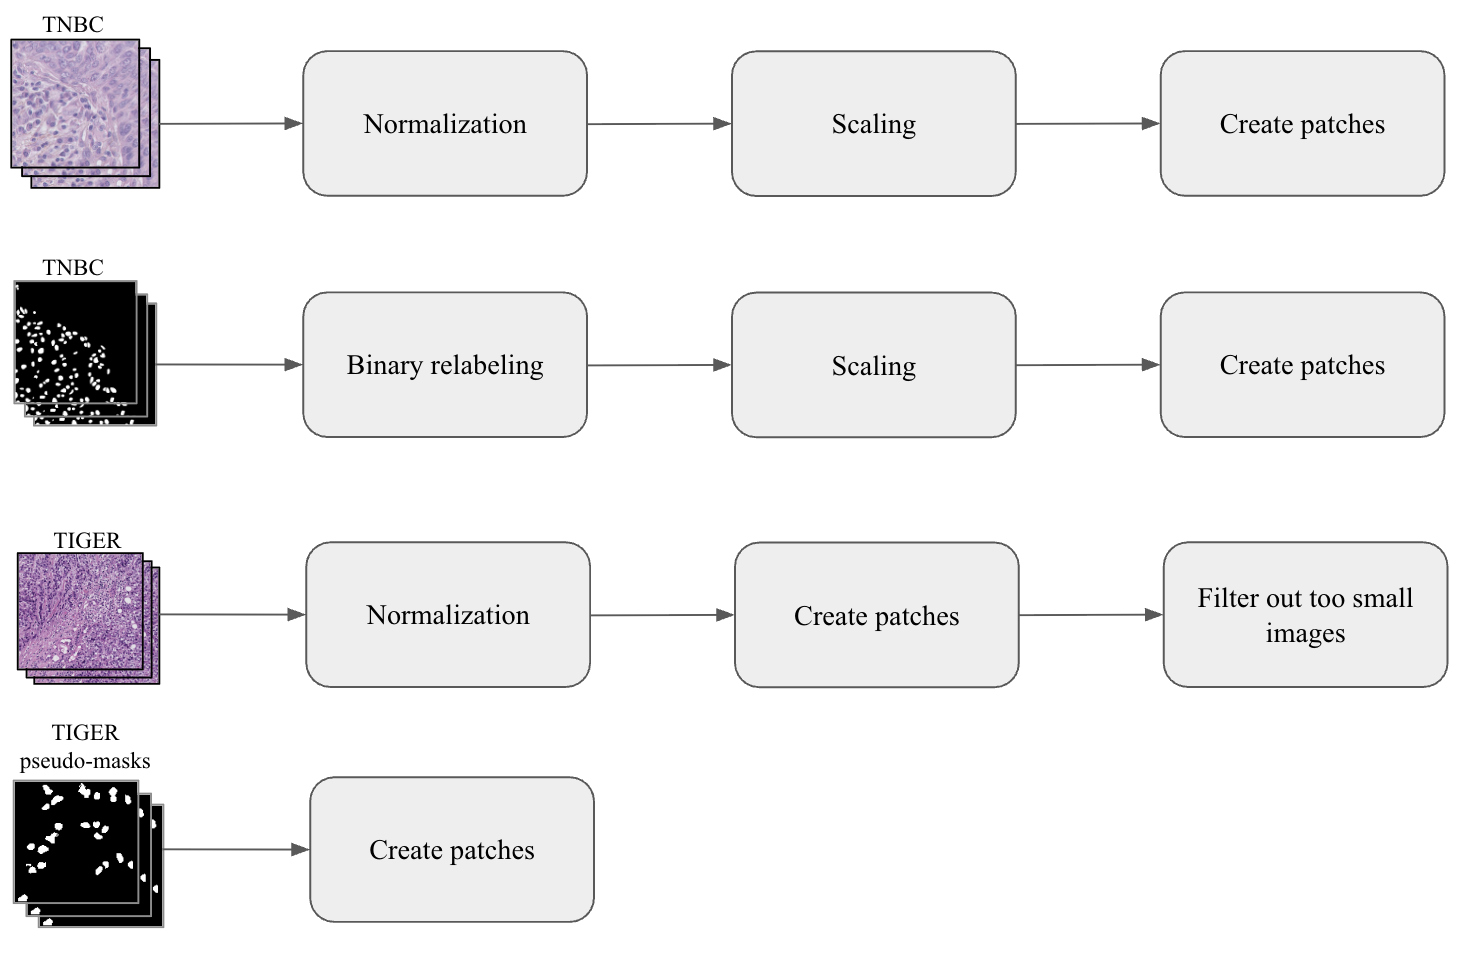
\includegraphics[width=\textwidth]{assets/images/for_presentation/dg-preprocessing.png}
\par\end{centering}
\caption{The preprocessing pipelines of both TIGER and TNBC datasets.
\label{fig:dg-preprocessing}}
\end{figure}

\subsection{Normalization} 
TIGER and TNBC datasets pose several challenges to us. As we described in section \ref{sec:datasets}, data come from four distinct sources (three for TIGER and one for TNBC) - this means that the staining is very different, which we can see in Figure \ref{fig:mix-no-norm}.

% Image
\begin{figure}[H]
  \centering
  % First row (2 images)
  \begin{subfigure}[b]{0.32\textwidth}
    \centering
    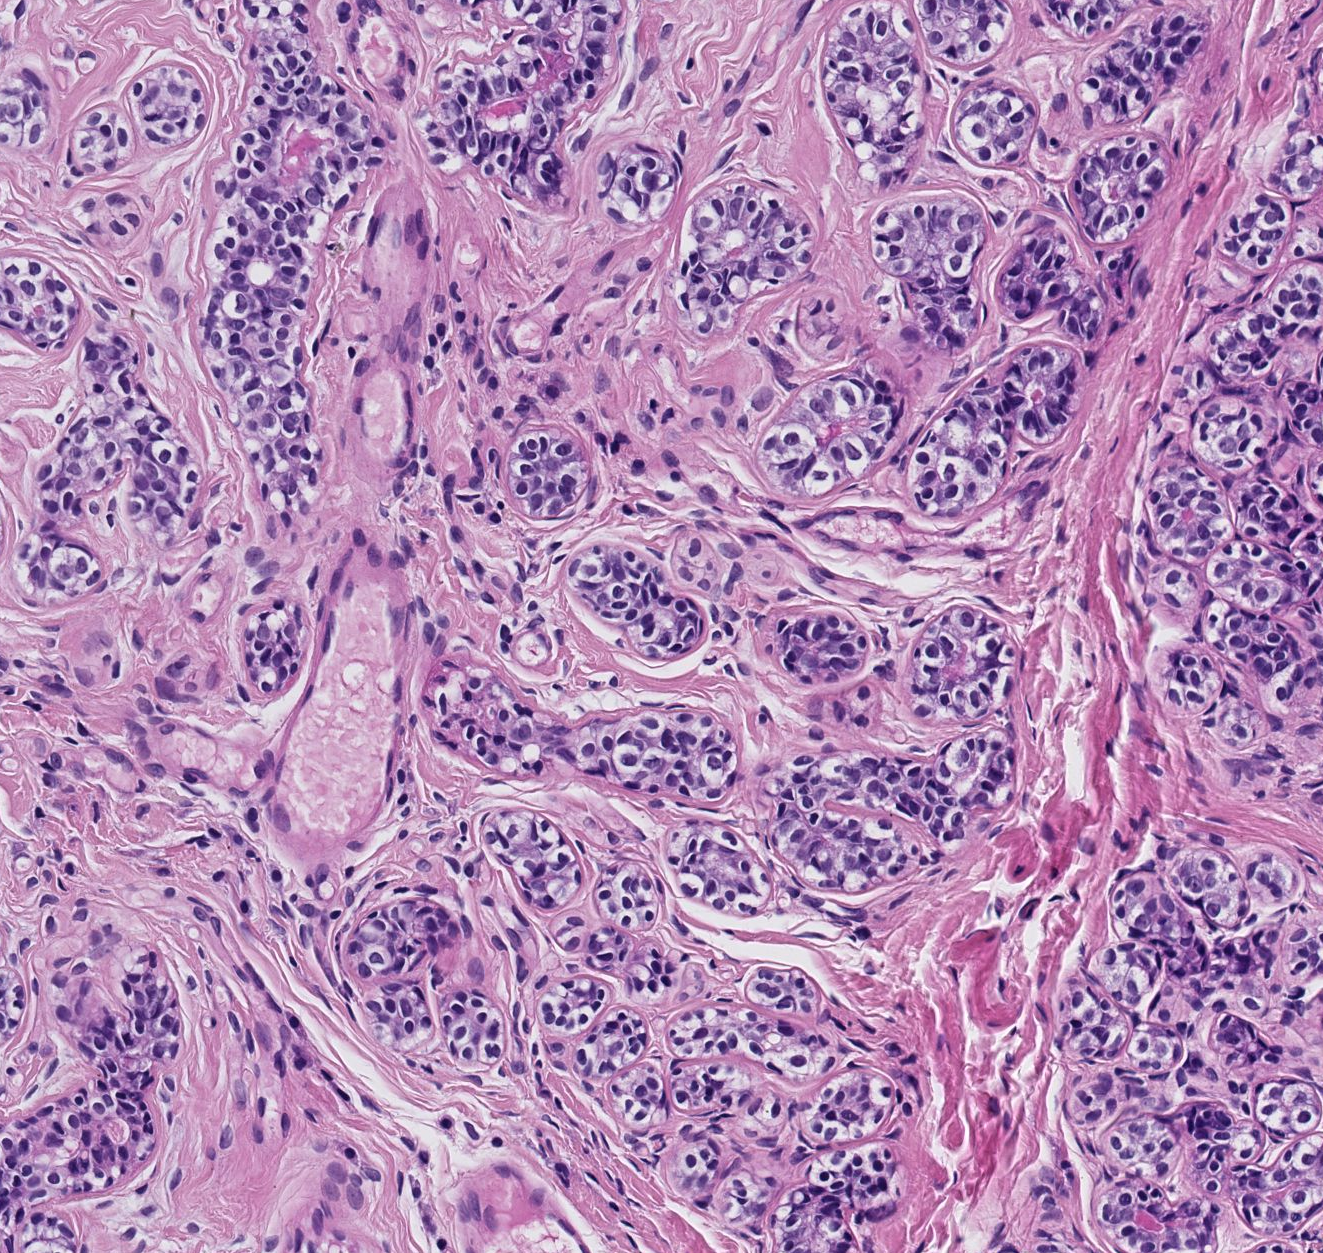
\includegraphics[width=\linewidth]{assets/images/for_presentation/image_100B_[10779, 11621, 12102, 12874].png}
    \caption{TIGER image – JB}
  \end{subfigure}\quad
  \begin{subfigure}[b]{0.32\textwidth}
    \centering
    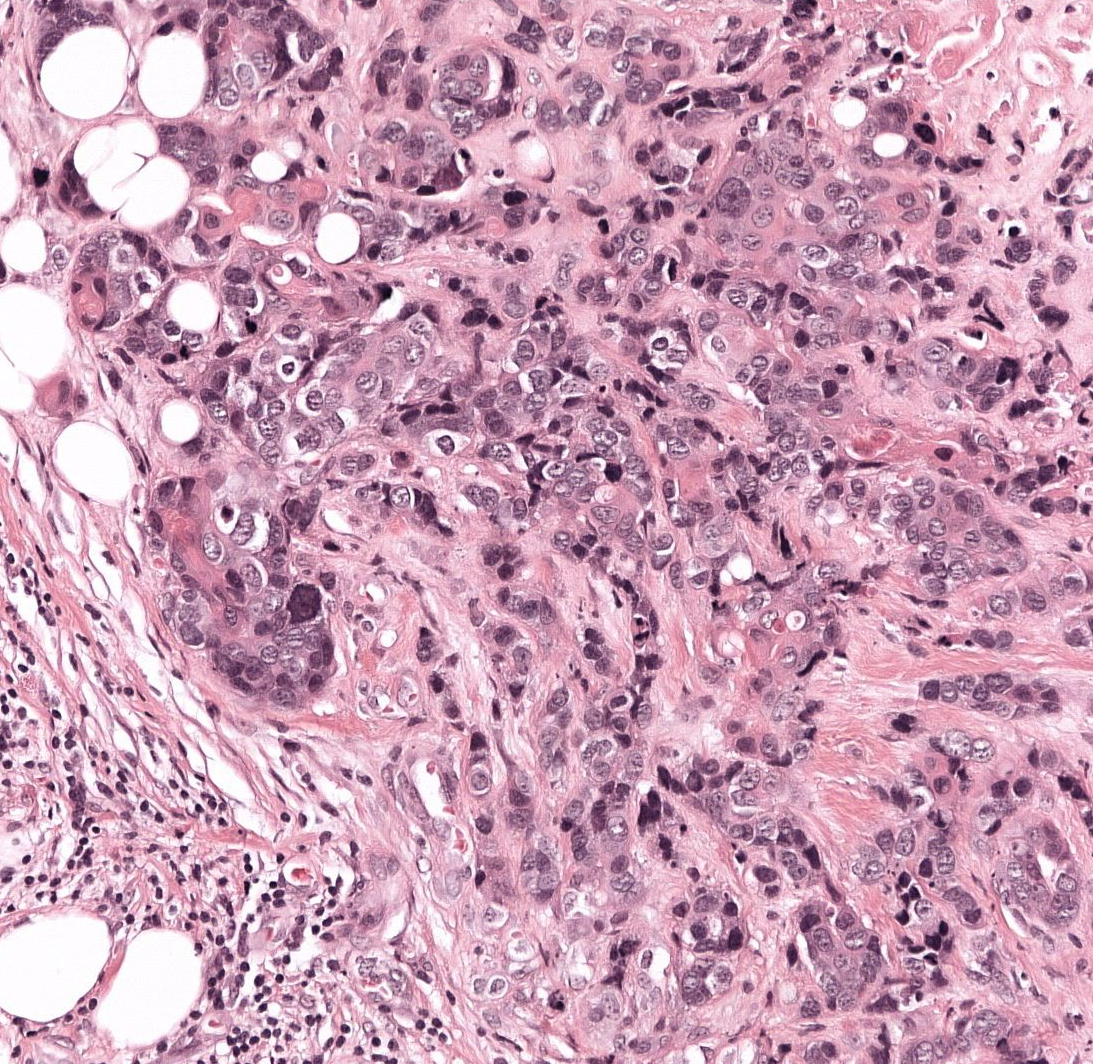
\includegraphics[width=\linewidth]{assets/images/for_presentation/image_TC_S01_P000003_C0001_B104_[50106, 52730, 51199, 53794].png}
    \caption{TIGER image – TC}
  \end{subfigure}

  \par\vspace{0.5em} % line break with a little vertical space

  % Second row (2 images)
  \begin{subfigure}[b]{0.32\textwidth}
    \centering
    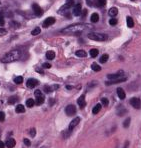
\includegraphics[width=\linewidth]{assets/images/for_presentation/image_TCGA-EW-A1P8-01Z-00-DX1.E9852193-8CDD-49EF-B49B-DA6931198F0D_[8391, 13690, 8532, 13838].png}
    \caption{TIGER image – TCGA}
  \end{subfigure}\quad
  \begin{subfigure}[b]{0.32\textwidth}
    \centering
    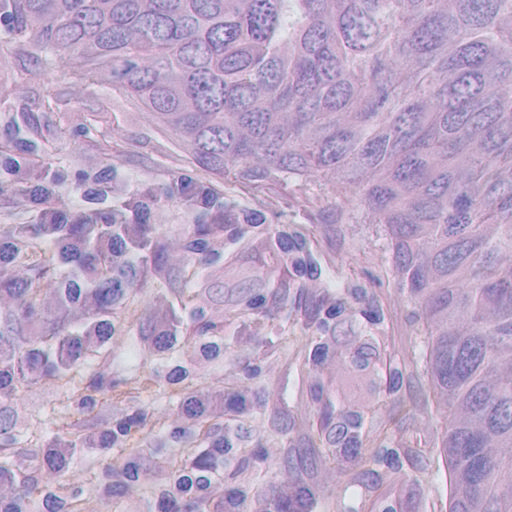
\includegraphics[width=\linewidth]{assets/images/for_presentation/image_10_1.png}
    \caption{TNBC image}
  \end{subfigure}

  \caption{Example images from TIGER datasets \cite{tiger_dataset} and TNBC \cite{TNBC-nuclei-seg-extended} before normalization.}
  \label{fig:mix-no-norm}
\end{figure}

Firstly, we tried a randomly selected single image as a reference image for Macenko normalization, which yielded suboptimal results when assessed visually. We have considered other approaches to selecting a reference image, but as a recent study \cite{Ivanov2024} showed, when selecting only a single reference image for Macenko normalization, the results will always be biased and suboptimal. Therefore, we employ the multi-target Macenko stain normalization technique as described in \cite{Ivanov2024}, where we select 8 reference images from the TIGER and 2 reference images from the TNBC dataset. This number is not arbitrary; in \cite{Ivanov2024}, authors experimented with a different number of reference images (2-20) and showed that the higher number has slightly better results, but if the number is too high, there are no significant improvements. They also experimented with different ways of computing the stain matrix, and the best results were achieved by the \textit{avg-post} method, and this method peaked when 10 reference images were selected \cite{Ivanov2024}. Given the sizes of our respective datasets, we decided to go with the 8 and 2 images and also with the \textit{avg-post} method. Then we used the same 10 reference images to normalize both datasets. The normalization technique improved the color inconsistencies, as we can see in Figure \ref{fig:mix-norm}.

\begin{figure}[H]
  \centering
  % First row (2 images)
  \begin{subfigure}[b]{0.32\textwidth}
    \centering
    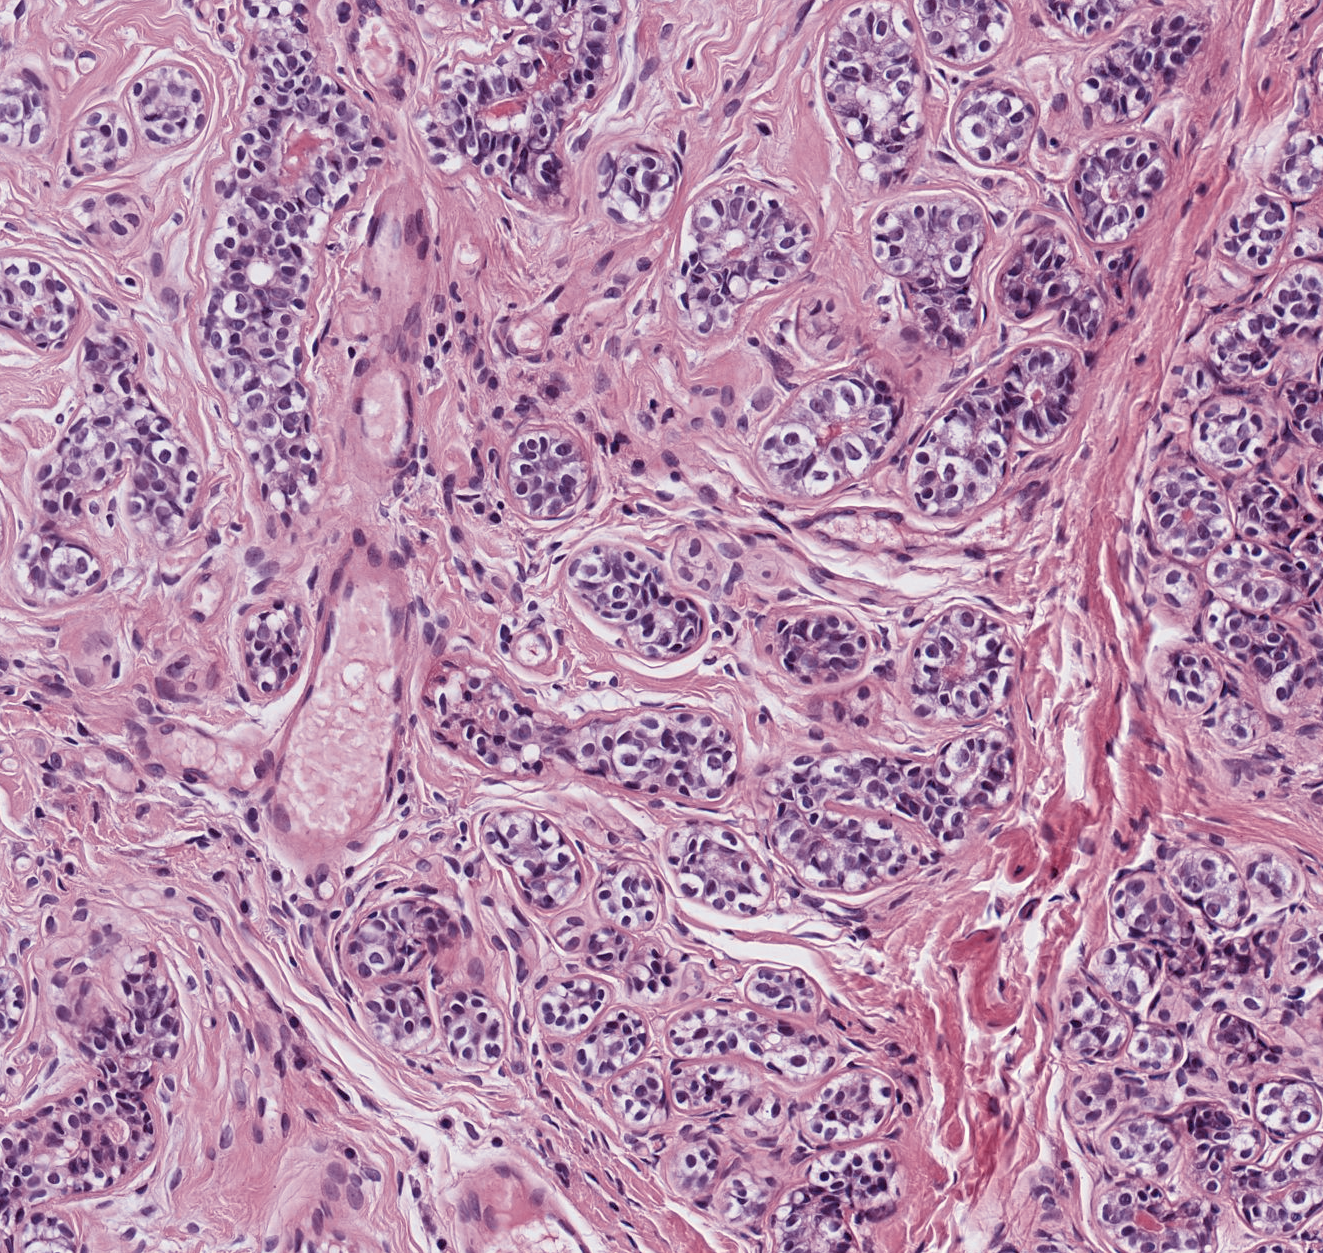
\includegraphics[width=\linewidth]{assets/images/for_presentation/norm_100B_[10779, 11621, 12102, 12874].png}
    \caption{TIGER image – JB}
  \end{subfigure}\quad
  \begin{subfigure}[b]{0.32\textwidth}
    \centering
    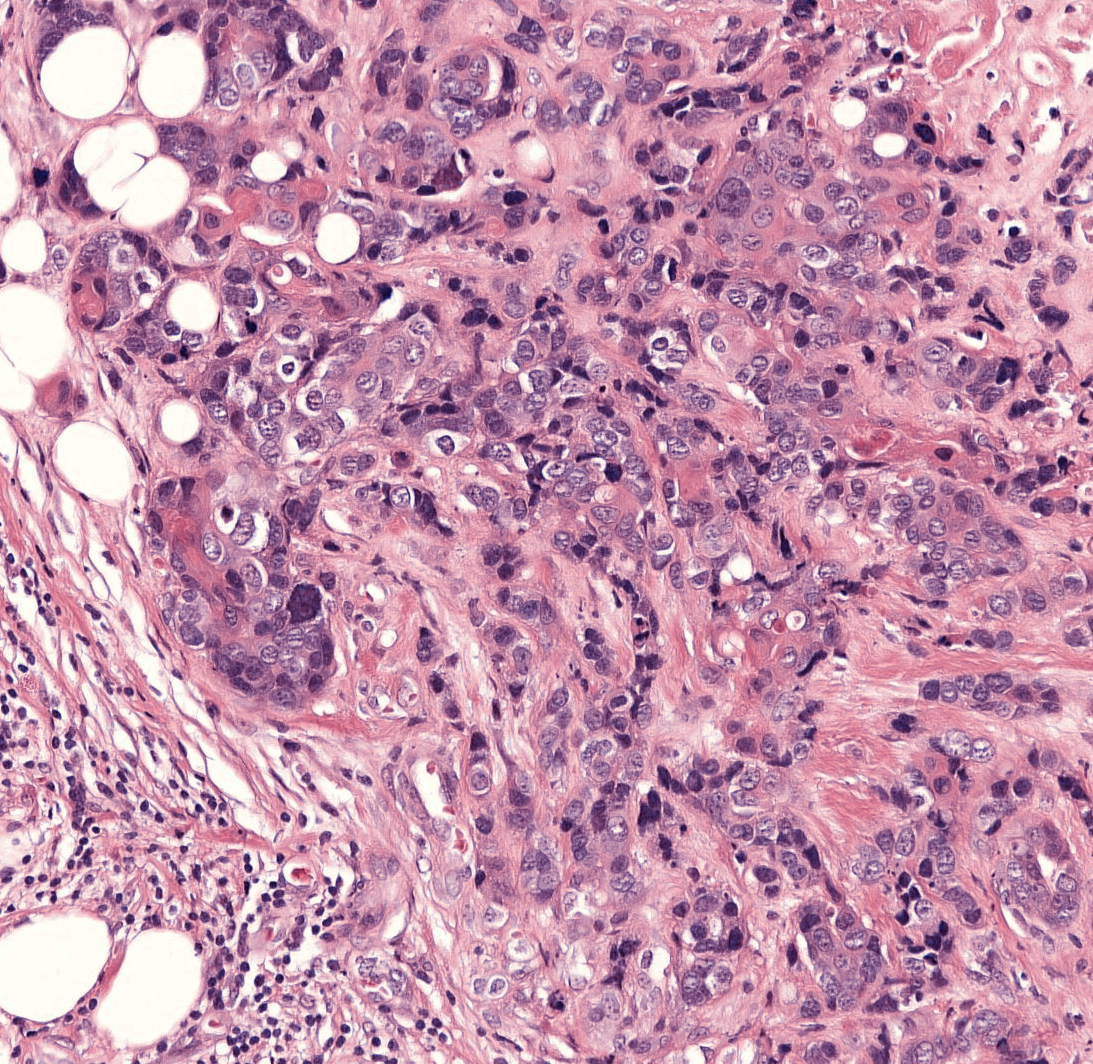
\includegraphics[width=\linewidth]{assets/images/for_presentation/norm_TC_S01_P000003_C0001_B104_[50106, 52730, 51199, 53794].png}
    \caption{TIGER image – TC}
  \end{subfigure}

  \par\vspace{0.5em} % line break with a little vertical space

  % Second row (2 images)
  \begin{subfigure}[b]{0.32\textwidth}
    \centering
    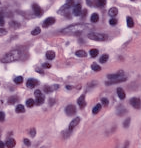
\includegraphics[width=\linewidth]{assets/images/for_presentation/norm_TCGA-EW-A1P8-01Z-00-DX1.E9852193-8CDD-49EF-B49B-DA6931198F0D_[8391, 13690, 8532, 13838].png}
    \caption{TIGER image – TCGA}
  \end{subfigure}\quad
  \begin{subfigure}[b]{0.32\textwidth}
    \centering
    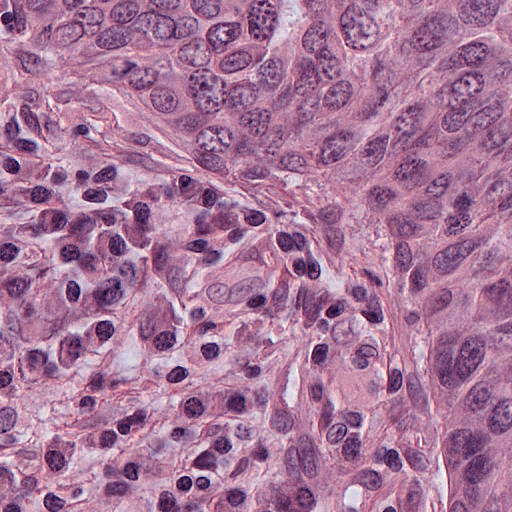
\includegraphics[width=\linewidth]{assets/images/for_presentation/norm_10_1.png}
    \caption{TNBC image}
  \end{subfigure}

  \caption{Example images from TIGER datasets \cite{tiger_dataset} and TNBC \cite{TNBC-nuclei-seg-extended} after normalization.}
  \label{fig:mix-norm}
\end{figure}

% Image

\subsection{Pseudo-mask sources} 
\label{subs:mask-sources}
The next step was to generate the pseudo-masks. For this, we created different variations of the same image. We named the images that were created as a part of one variation \textit{image source}. In total, six different image sources were created for the experiments. We used the original (raw) image as one source, then the normalized image as another source. Furthermore, we extracted the hematoxylin image out of the original image (Macenko normalization does this internally). This was done based on the fact that hematoxylin highlights the cell nuclei, as we described in Chapter \ref{chapter:intro}. This hematoxylin image became our third image source. Lastly, by applying histogram equalization to all of the aforementioned image sources (to increase the overall contrast of the image and shift dark colors into darker ones and light into lighter ones), we obtained another three image sources. The difference in the image sources can be seen in Figure \ref{fig:tiger-sources}. 

\begin{figure}[H]
  \centering
  % First row of three subfigures
  \begin{subfigure}[b]{0.32\textwidth}
    \centering
    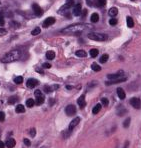
\includegraphics[width=\linewidth]{assets/images/for_presentation/image_TCGA-EW-A1P8-01Z-00-DX1.E9852193-8CDD-49EF-B49B-DA6931198F0D_[8391, 13690, 8532, 13838].png}
    \caption{Original image}\label{fig:tiger-raw}
  \end{subfigure}\hfill
  \begin{subfigure}[b]{0.32\textwidth}
    \centering
    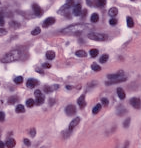
\includegraphics[width=\linewidth]{assets/images/for_presentation/norm_TCGA-EW-A1P8-01Z-00-DX1.E9852193-8CDD-49EF-B49B-DA6931198F0D_[8391, 13690, 8532, 13838].png}
    \caption{Normalized image}\label{fig:tiger-norm}
  \end{subfigure}\hfill
  \begin{subfigure}[b]{0.32\textwidth}
    \centering
    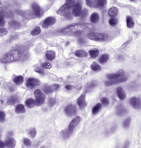
\includegraphics[width=\linewidth]{assets/images/for_presentation/hem_TCGA-EW-A1P8-01Z-00-DX1.E9852193-8CDD-49EF-B49B-DA6931198F0D_[8391, 13690, 8532, 13838].png}
    \caption{Hematoxylin image}\label{fig:tiger-hem}
  \end{subfigure}

  % Line break to start the second row; adjust vertical space as needed
  \par\vspace{0.5em}

  % Second row of three subfigures
  \begin{subfigure}[b]{0.32\textwidth}
    \centering
    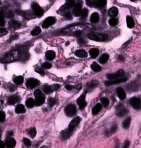
\includegraphics[width=\linewidth]{assets/images/for_presentation/eq_TCGA-EW-A1P8-01Z-00-DX1.E9852193-8CDD-49EF-B49B-DA6931198F0D_[8391, 13690, 8532, 13838].png}
    \caption{Original image with histogram equalization}\label{fig:tiger-eq}
  \end{subfigure}\hfill
  \begin{subfigure}[b]{0.32\textwidth}
    \centering
    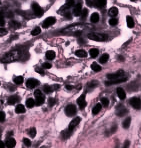
\includegraphics[width=\linewidth]{assets/images/for_presentation/norm_eq_TCGA-EW-A1P8-01Z-00-DX1.E9852193-8CDD-49EF-B49B-DA6931198F0D_[8391, 13690, 8532, 13838].png}
    \caption{Normalized image with histogram equalization}\label{fig:tiger-norm-eq}
  \end{subfigure}\hfill
  \begin{subfigure}[b]{0.32\textwidth}
    \centering
    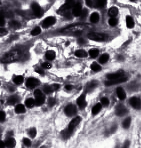
\includegraphics[width=\linewidth]{assets/images/for_presentation/hem_eq_TCGA-EW-A1P8-01Z-00-DX1.E9852193-8CDD-49EF-B49B-DA6931198F0D_[8391, 13690, 8532, 13838].png}
    \caption{Hematoxylin image with histogram equalization}\label{fig:tiger-hem-eq}
  \end{subfigure}
  \caption{Examples of image sources.}
  \label{fig:tiger-sources}
\end{figure}


We then operated on each image source with different computer vision techniques to generate the final pseudo-mask PNGs. We describe each of these techniques in Section \ref{section:mask-generation}. 

\subsection{Aligning the TNBC dataset} 
To use the TNBC dataset, we needed to align its scale and the ground truth masks. This dataset was scanned with the $40\!\times\!$ magnification; however, the TIGER dataset was scanned using the $20\!\times\!$ magnification. To align them, we down-scaled the TNBC dataset images and masks by a factor of 2. Moreover, the TNBC ground truth masks were relabeled to binary masks by setting all of the other labels except for the lymphocyte cell labels as background.

\subsection{Patching Strategy}
To be able to feed our data to the deep learning UNet model, we created patches of fixed size $128\!\times\!128$ pixels. The TIGER dataset contained images of varying sizes. Therefore, we created overlapping patches with a dynamic stride in such a way that no patch was shifted outside of the original image. We created 19,386 patches of the TIGER dataset images. The TNBC dataset was nicer since the original images were of $512\!\times\!512$ pixels in size, and after down-scaling by a factor of 2, they became $256\!\times\!256$ pixels. Each image was then split into 4 non-overlapping patches. This got us exactly 200 patches of TNBC dataset images. After this stage, the data is ready for the training and evaluation process.

\subsection{Images to Tensors}
For the PyTorch framework to work with the PNG image patches, both original images and masks, we needed to convert them from NumPy arrays into tensors. This was done before the training and evaluation of each trained model.

\section{Pseudo-masks Generation}
\label{section:mask-generation}
To be able to start training the segmentation model on the TIGER dataset, we needed to convert the bounding box annotations of lymphocyte nuclei into pixel-level pseudo-masks. We used a series of computer vision methods, which were chained in different ways to better identify the region where a cell nucleus is present within the bounding box. This task was challenging because of the lower contrast between the nuclei and the surrounding tissue, and also because some nuclei were too close to each other, meaning that there was an overlap between the bounding boxes. This inspired us to create different versions of a single image, to promote some properties of the image, such as increasing the contrast or isolating only the hematoxylin staining. We called these versions image sources, and the process of their creation is described in Subsection \ref{subs:mask-sources} as a part of image preprocessing. The whole process of pseudo-mask generation can be seen in Figure \ref{fig:dg-mask-gen}. To better understand the chain of operations applied, we will illustrate it on a single image example of one image source:

\begin{enumerate}
    \item Firstly, the image is loaded together with its corresponding bounding box annotations.
    \item Next, the individual labeled nuclei are cropped out of the image, using the bounding box values.
    \item Then a four combinations of operations are applied on the cropped region, which means that from the single cropped region, four new versions of it are created, based on which combination of operations was applied. It was either:
    \begin{itemize}
        \item The Otsu thresholding
        \item The Adaptive thresholding
        \item The median blur with Otsu thresholding
        \item The median blur Adaptive thresholding
    \end{itemize}
    \item In the next step, the morphological opening is applied to remove small artifacts left after the thresholding.
    \item The previous operations created so far a 'prototype' of the pseudo-mask. In the subsequent step, the marked watershed is applied, which uses this prototype together with the initial cropped image region to create a final pseudo-mask.
    \item Finally, the small pseudo-masks for individual cells are combined into a full-image pseudo-mask
\end{enumerate}

\begin{figure}[H]
\begin{centering}
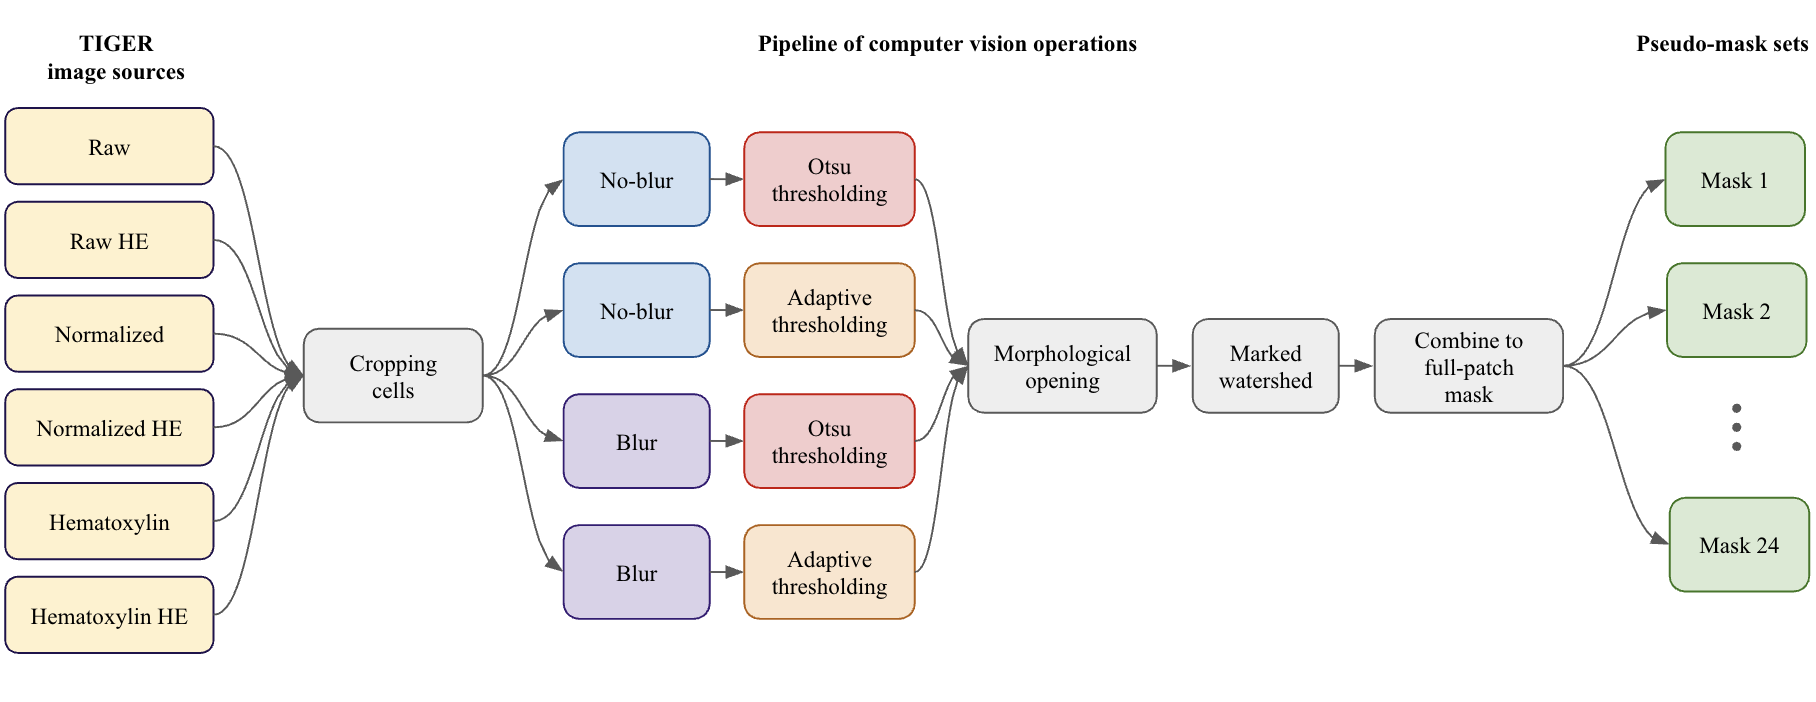
\includegraphics[width=\textwidth]{assets/images/for_presentation/dg-mask-gen.png}
\par\end{centering}
\caption{The process of pseudo-masks generation. 
\label{fig:dg-mask-gen}}
\end{figure}

Given that we work with 6 image sources and 4 pipelines of computer vision operations, where each pipeline is applied to every image source, this gives us in total of 24 pseudo-masks for any given image. In the following paragraphs, we describe each computer vision operation in more detail.

\paragraph{Median Blur}
We use the $3\!\times\!3$ median blur with the intuition that it could remove small noises around the cell nuclei. This filter replaces each pixel with the median of its neighborhood, which is determined by the size of the kernel. We use the kernel of size $3\!\times\!3$ - this is reasonable for us, since the bounding boxes are of size $12\!\times\!12$, $16\!\times\!16$, or $18\!\times\!18$ and we do want to remove possible small noise but still preserve the shape of the nuclei.

\paragraph{Otsu Thresholding}
The Otsu thresholding finds a threshold that minimizes intra-class variance and then binarizes the pixel values based on this threshold. Since this operation needs a grayscale image, we first do this conversion. Then we apply the Otsu thresholding method and inversion - this automatically computes the optimal Otsu threshold and also inverts the binarization so that dark nuclei appear as white foreground and background pixels become black.

\paragraph{Adaptive Thresholding}
In contrast to Otsu thresholding, adaptive thresholding computes the threshold for each pixel based on its neighborhood. We use the $11\!\times\!11$ adaptive thresholding with a constant of 2 - this ensures that we cover the small nuclei diameter but still preserve fine details. In the Equation \ref{eq:adaptive} we can see how the threshold $T(x,y)$ is computed for each pixel with coordinates $x$ and $y$. Firstly, a window $\mathcal{W}$ of size $B\!\times\! B$ is centered around the pixel. Then each pixel's grayscale intensity $I(u,v)$ within this window with pixel coordinates $u$ and $v$ is summed and then averaged. Finally, a constant is subtracted from this mean to bias the threshold below the local mean. Again, we use it with inversion, as in Otsu thresholding.

\begin{align}
\label{eq:adaptive}
T(x,y)
=
\frac{1}{B^2}
\sum_{u = x - \frac{B-1}{2}}^{\,x + \frac{B-1}{2}}
\;\;
\sum_{v = y - \frac{B-1}{2}}^{\,y + \frac{B-1}{2}}
I(u,v)
\;-\; C
\end{align}

\paragraph{Morphological Opening}
We use the elliptical $3\!\times\!3$ morphological opening to remove any small artifacts left after the thresholding operations and to preserve the shape of the nuclei.

\paragraph{Marked Watershed}
To obtain the final pseudo-mask, we employ the mark-controlled watershed. This includes a series of steps:
\begin{enumerate}
    \item Firstly, the distance transform operation computes, for each foreground pixel in the so-far-created binary mask, the Euclidean distance to the nearest background pixel, producing a map whose peaks lie at object centers.
    \item Secondly, we threshold the distance map, which keeps only the central ~30\% of each cell nucleus - this helps to separate the touching nuclei and gives us the pseudo-mask of sure foreground area (the sure nuclei area).
    \item Then we dilate the sure foreground with a $3\!\times\!3$ elliptical kernel to expand the region. Now we consider all pixels lying outside of these regions as sure background.
    \item After that, we subtract the sure foreground from the sure background mask. This gives us the regions that should have the shape of a ring and are 'unknown' - either background or foreground. Those are the pixels that lie on the boundaries of each cell.
    \item Next, we do marker labeling - we mark each connected component of the sure foreground mask with a different mark (integer), starting with number 1. Then we add number 1 to each pixel value. Lastly, we set those pixels that are marked as an unknown region to zero. This step ensures that:
    \begin{itemize}
        \item The sure foreground areas start from number 2 onward,
        \item The sure background areas are marked with number 1, and
        \item The unknown regions are marked with number 0.
    \end{itemize}
    \item Finally, the watershed algorithm will flood and try to segment the unknown regions (marked with 0). It treats the original image provided to it (the colorful crop of cell nuclei) as a height map, where the brighter pixels represent high elevations and the darker pixels represent low elevations. It also uses the marker image to seed the foreground and background regions. During the segmentation process, it floods the image starting at each marker label, and when the floods meet, the lines separating the cell nuclei are created. Pixels on these delineating lines have a value set to -1.
\end{enumerate}

After the mark-controlled watershed produces the delineated nuclei mask, we set all pixel values that are lower than or equal to 1 to 0 (sure background and delineation lines) and those that are greater than 1 (all nuclei components) to 1 to create a binary pseudo-mask.

\paragraph{Full-patch Combining}
After we obtain the small-sized pseudo-masks for each cell nucleus bounding box, we reconstruct the full-patch mask by firstly creating an image where all pixels have 0 values and then applying the binary OR operation with the small-sized pseudo-masks on the position from which they were cropped. By this, we get the final pseudo-mask for the original image, where pixels of nuclei regions have values of 1 and background pixels have values of 0.

\section{Pseudo-masks Fusion}
\label{section:mask-fusion}
During the generation of pseudo-masks, we obtained 24 different masks per single image. We decided to fuse them based on the results of the experiment, which we present in Subsection \ref{sub:exp-2} and based on the visualization of the combined masks, which we can see in Figure \ref{fig:combined-vis}. These combined masks were created using the pixel-wise addition of all 24 pseudo-masks, which gave us a single pseudo-mask per image, where pixel values ranged between 0 (all pseudo-masks labeled the pixel as background) and 24 (all masks labeled the pixel as foreground). For visualization, a pixel-wise multiplication by 10 was applied to the resulting pseudo-masks to better see the combined power of the pseudo-masks.

\begin{figure}[H]
  \begin{subfigure}[b]{0.24\textwidth}
    \centering
    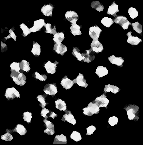
\includegraphics[width=\linewidth]{assets/images/for_presentation/combined-1.png}
  \end{subfigure}\hfill
  \begin{subfigure}[b]{0.24\textwidth}
    \centering
    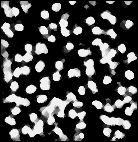
\includegraphics[width=\linewidth]{assets/images/for_presentation/combined-2.png}
  \end{subfigure}\hfill
  \begin{subfigure}[b]{0.24\textwidth}
    \centering
    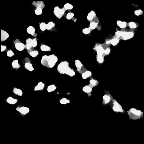
\includegraphics[width=\linewidth]{assets/images/for_presentation/combined-3.png}
  \end{subfigure}
  \begin{subfigure}[b]{0.24\textwidth}
    \centering
    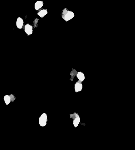
\includegraphics[width=\linewidth]{assets/images/for_presentation/combined-4.png}
  \end{subfigure}
  \caption{Examples of combined pseudo-masks.}
  \label{fig:combined-vis}
\end{figure}

We decided to try two different fusion approaches:

\begin{enumerate}
  \item Fuse the pseudo-masks via pixel-wise voting at quartile agreement levels - 100\%, 75\%, 50\%, and 25\% - keeping only those pixels declared foreground by at least that percentage of the masks which achieved the highest Dice scores in the experiment of Subsection~\ref{sub:exp-2}. This gave us four sets of fused masks. The overview of this fusing approach can be seen in Figure \ref{fig:dg-mask-fuse-2}. Firstly, the masks are summed together (pixel-wise) and then all pixels that are greater than 0 are set to 1 (foreground - nuclei) to maintain the binary mask.
  \item Fuse the pseudo-masks via pixel-wise voting consensus by all involved masks - a pixel was labeled as foreground (cell nuclei) if either:
  \begin{itemize}
      \item 24 out of 24 masks declared the pixel as foreground,
      \item 23 out of 24 masks declared the pixel as foreground,
      \item 22 out of 24 masks declared the pixel as foreground, or
      \item 21 out of 24 masks declared the pixel as foreground.
  \end{itemize}
  This approach also gave us another four sets of fused masks. The whole process can be seen in Figure \ref{fig:dg-mask-fuse-1}. We always use all 24 pseudo-mask sets, sum the pseudo-masks (pixel-wise), and then the threshold is used based on the voting strategy. If the pixel value is greater than or equal to the number of masks that need to agree on it (either 24, 23, 22, or 21), it is set to 1 (foreground - nuclei); otherwise, it is set to 0 (background).
\end{enumerate}

Together, we obtained 8 sets of fused masks.

\begin{figure}[H]
\begin{centering}
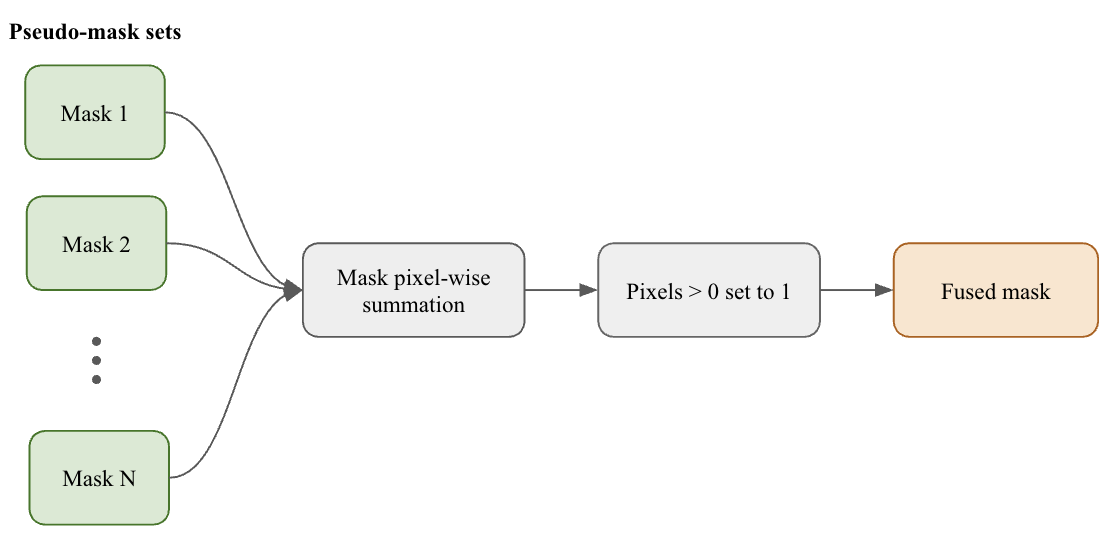
\includegraphics[width=\textwidth]{assets/images/for_presentation/dg-mask-fuse-2.png}
\par\end{centering}
\caption{The process of pseudo-masks fusion using quartile agreement levels.
\label{fig:dg-mask-fuse-2}}
\end{figure}

\begin{figure}[H]
\begin{centering}
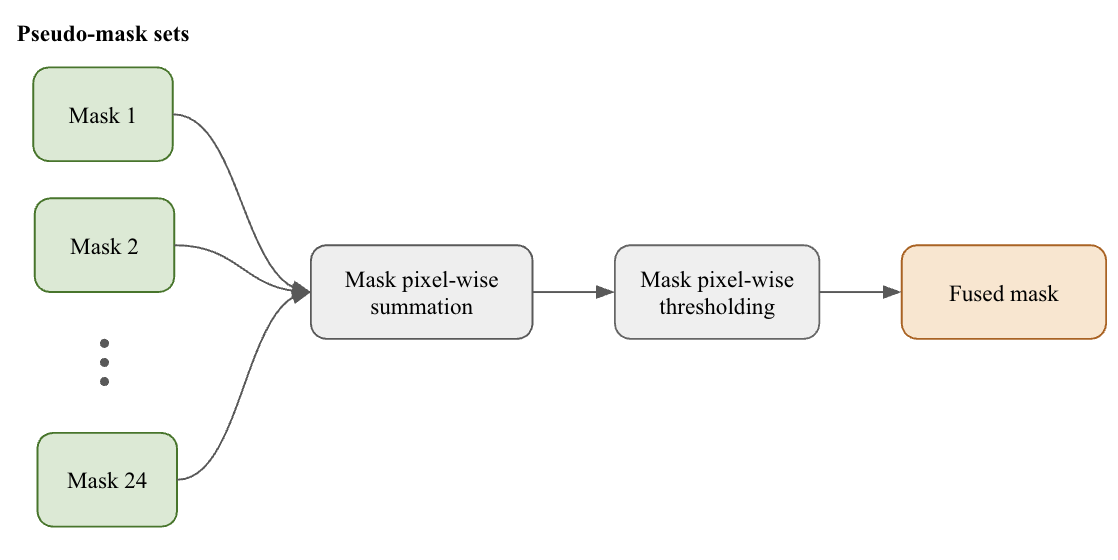
\includegraphics[width=\textwidth]{assets/images/for_presentation/dg-mask-fuse-1.png}
\par\end{centering}
\caption{The process of pseudo-masks fusing using voting consensus. 
\label{fig:dg-mask-fuse-1}}
\end{figure}

\section{Experiments}
\label{section:experiments}
Our proposed system evolved with each performed experiment, since each experiment built on the previous one. We will describe each experiment in this section, with a focus on the data used for training and testing, the experiment setup and workflow, and the results of the experiment. Every experiment was run three times to reduce the risk that random initialization of the model's parameters, or the split of training data into training and validation subsets, would significantly improve or significantly worsen the final results.

For the first experiment, we utilized just the U-Net model itself as a deep learning module. The fully annotated TNBC dataset was used for this task.

The second experiment used the pseudo-masks generated by a combination of image sources and different computer vision techniques. The pseudo-masks were generated for the weakly annotated TIGER dataset from the provided bounding box annotations. These were then used as ground truth masks for subsequent training of the U-Net model, which was trained on the TIGER dataset. For the final evaluation, the TNBC dataset was used.

The third experiment builds on the second. It compared the different fusing strategies of mask sets. Again, we used these fused masks to train the U-Net model on the TIGER dataset, and the TNBC dataset was used for the final evaluation.

In the fourth experiment, we utilized a transfer learning strategy, where we took the best model trained during the third experiment and fine-tuned it using part of the fully annotated TNBC dataset.

\subsection{Experiment 1 - Training on TNBC Dataset}
\label{sub:exp-1}
In the first experiment, we wanted to check whether the small, fully annotated TNBC dataset would be sufficient for training the segmentation model.

\paragraph{Data}
We use only the fully annotated TNBC dataset, both for the training and for the final evaluation. This dataset is split into three folds, where the folds contain the following number of image patches:

\begin{itemize}
    \item Fold 1 contains 72 image patches, from 4 patients,
    \item Fold 2 contains 68 image patches, from 4 patients, and
    \item Fold 3 contains 60 image patches, from 3 patients
\end{itemize}

Always, two folds were used as the training set, and one fold was used as the testing set. Together, this gave us three rounds of training and evaluation for one experiment run. To calculate the final result for each reported metric, the weighted average of the metrics logged by every round was calculated, given the Equation \ref{eq:weighted_avg}, where $\bar{M}$ is the final reported metric (Dice coefficient and IoU), $n$ is the number of the fold that was used for evaluation, $i$ is the \textit{i}-th fold used for model evaluation, $M_i$ is the evaluation metric calculated when evaluating the model on the \textit{i}-th fold, and $W_i$ is the size of the \textit{i}-th fold.

\begin{align}
\label{eq:weighted_avg}
\bar{M} &= \frac{\sum_{i=1}^{n} M_i \cdot W_i}{\sum_{i=1}^{n} W_i}
\end{align}

The run of this experiment is simple. We train the U-Net model using the TNBC dataset, with the provided ground truth masks, and evaluate it on the same dataset.

\paragraph{Results}
The experiment ran on average around 35 epochs due to early stopping. From the training and validation loss in Figure \ref{fig:exp1-loss}, we can observe that the model was not able to learn when trained only on the small, although fully annotated, dataset. This can be seen both in the graph spikes on the training loss as well as on the validation loss, which was not able to improve significantly after the first 10 epochs. We see this also on the evaluation metrics, which are summarized in Table \ref{tab:exp1-metrics}, where the Dice coefficient was 18.91\% and the IoU was 10.64\%. In the Figure \ref{fig:exp1-results}, we can see that the model was not able to differentiate between different cell nuclei types, nor was it able to distinguish the cell nuclei and the background area.

\begin{table}[H]
\centering
\begin{tabular}{ p{5.0cm} | p{5.0cm} }
\hline
\textbf{Metric} & \textbf{Value (\%)} \\ 
\hline
Dice coefficient &  18.91 \\ 
IoU &  10.64 \\ 
\hline
\end{tabular}
\caption{Results of the model trained on the TNBC dataset.}
\label{tab:exp1-metrics}
\end{table}

\begin{figure}[H]
\begin{centering}
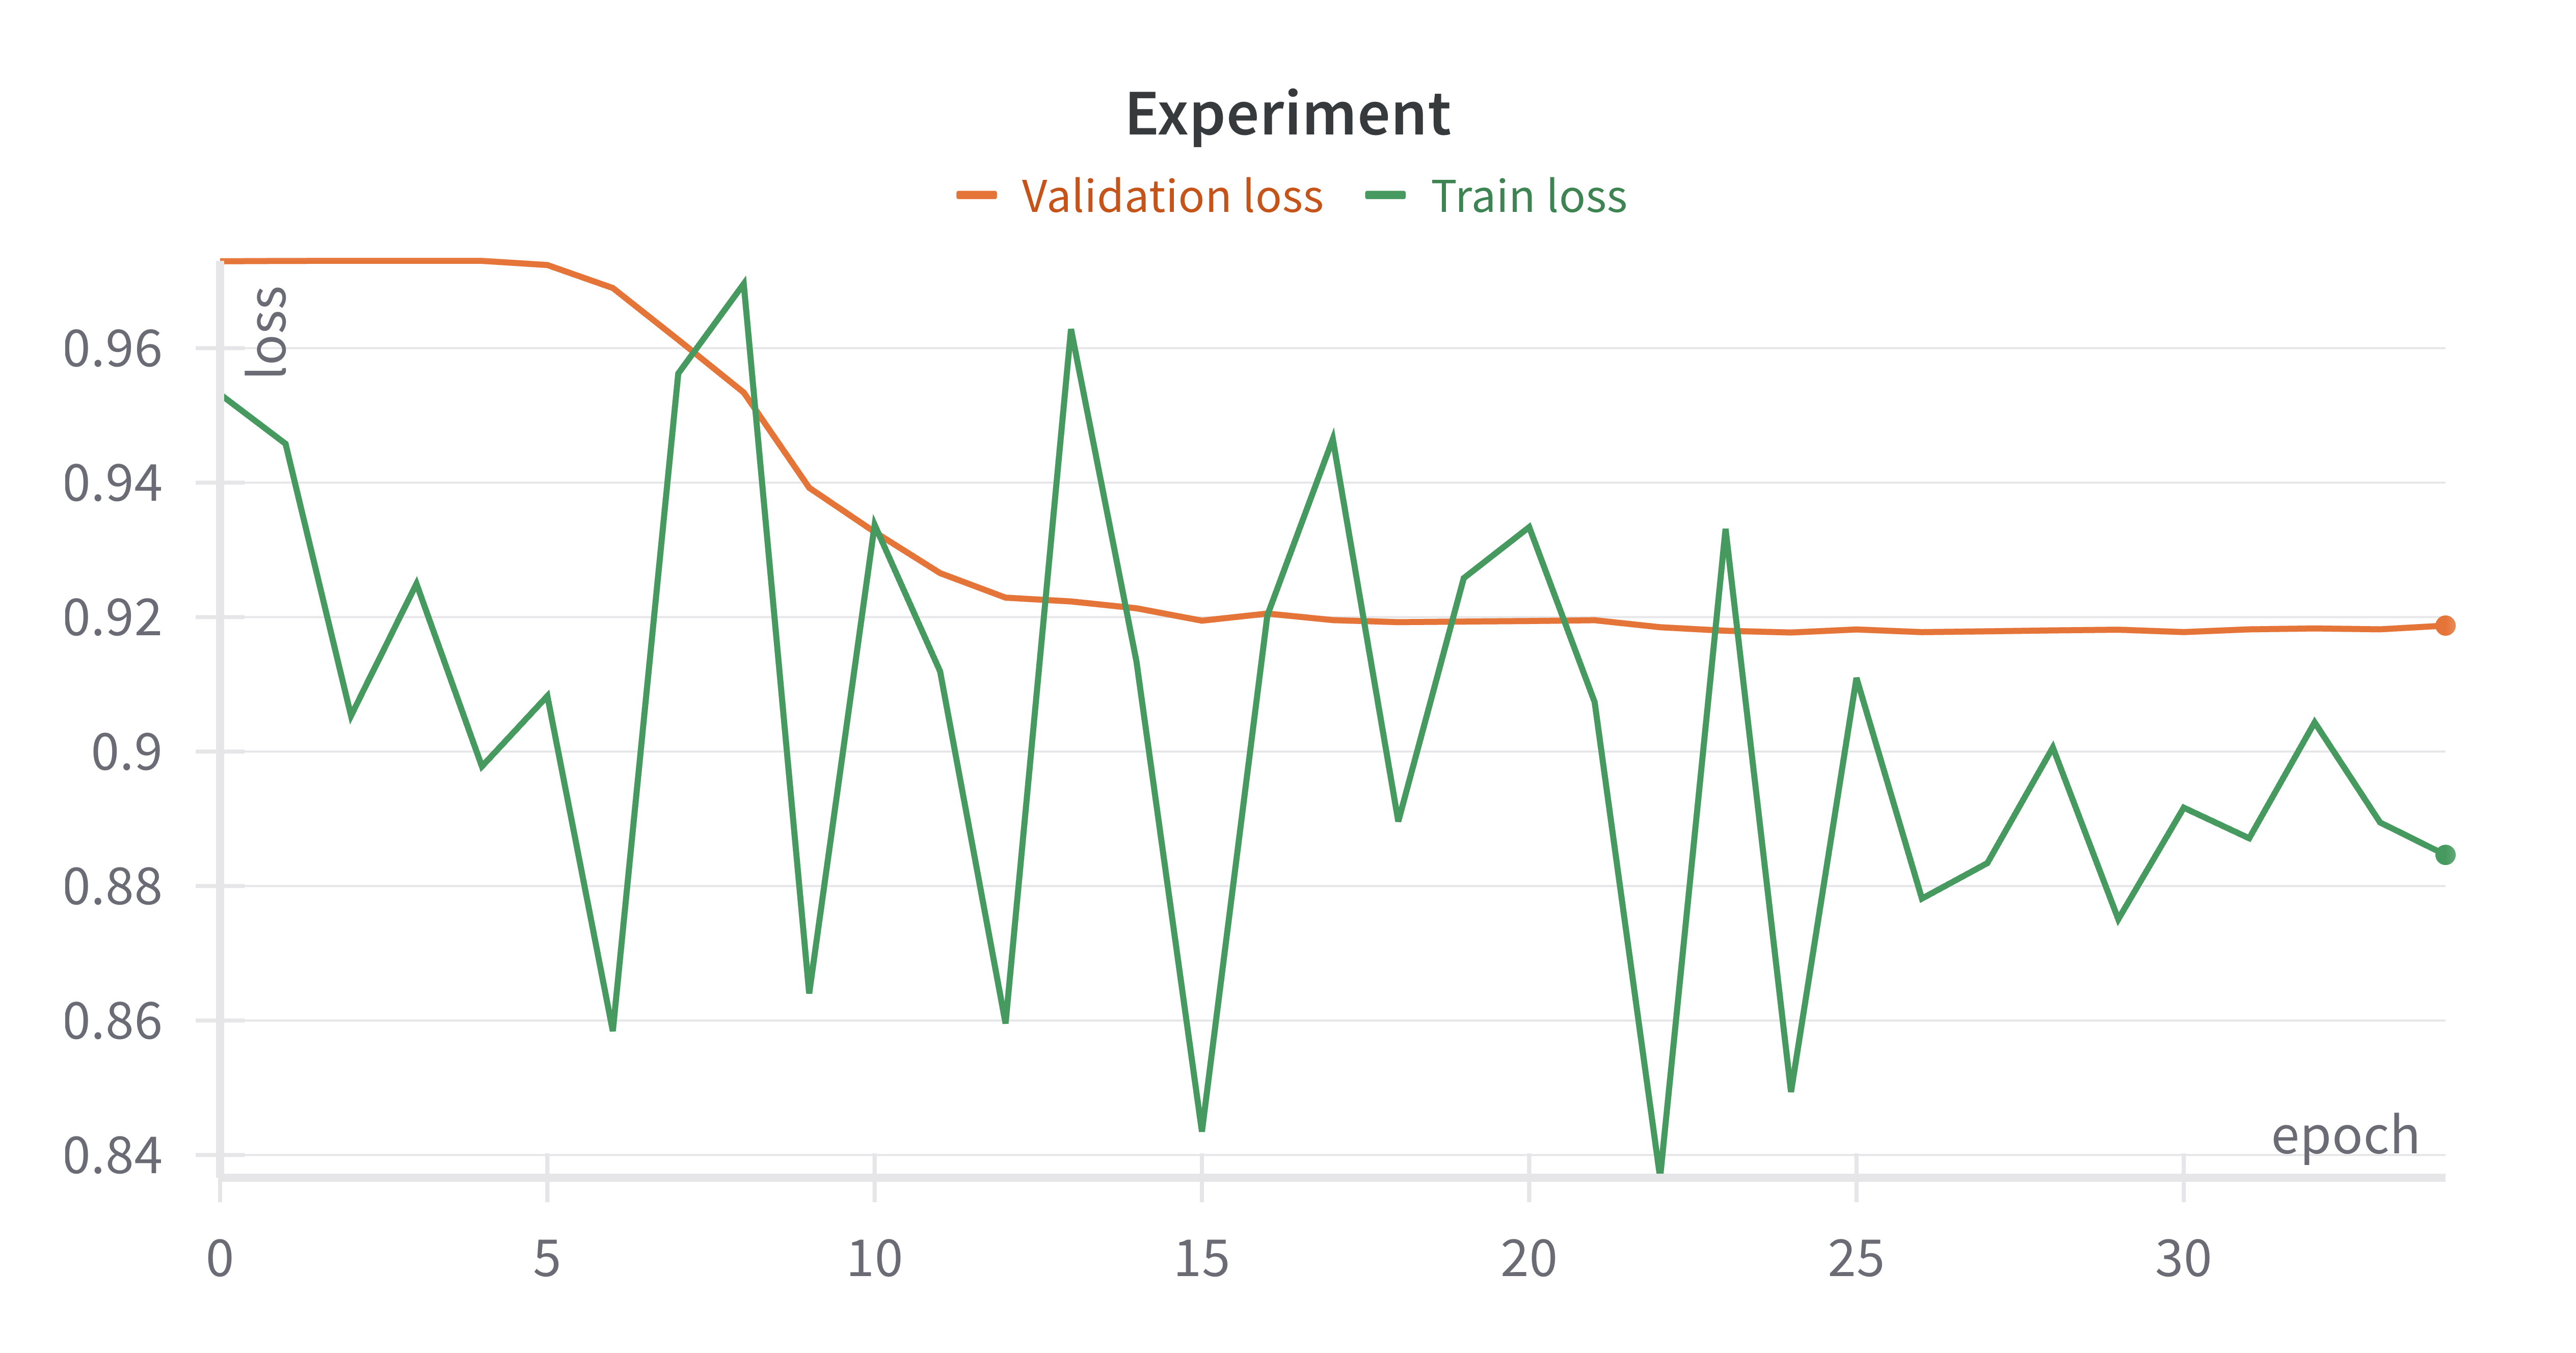
\includegraphics[width=\textwidth]{assets/images/for_presentation/exp1-loss.png}
\par\end{centering}
\caption{The loss function during training (green) and validation (orange) of the model trained on the TNBC dataset.
\label{fig:exp1-loss}}
\end{figure}

\begin{figure}[H]
  \centering
  % First row of three subfigures
  \begin{subfigure}[b]{0.32\textwidth}
    \centering
    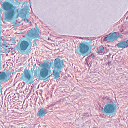
\includegraphics[width=\linewidth]{assets/images/for_presentation/exp1-1-pred.png}
    \caption{Image 1 prediction}
  \end{subfigure}\hfill
  \begin{subfigure}[b]{0.32\textwidth}
    \centering
    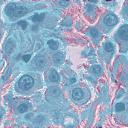
\includegraphics[width=\linewidth]{assets/images/for_presentation/exp1-2-pred.png}
    \caption{Image 2 prediction}
  \end{subfigure}\hfill
  \begin{subfigure}[b]{0.32\textwidth}
    \centering
    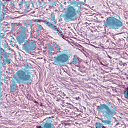
\includegraphics[width=\linewidth]{assets/images/for_presentation/exp1-3-pred.png}
    \caption{Image 3 prediction}
  \end{subfigure}

  % Line break to start the second row; adjust vertical space as needed
  \par\vspace{0.5em}

  % Second row of three subfigures
  \begin{subfigure}[b]{0.32\textwidth}
    \centering
    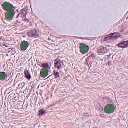
\includegraphics[width=\linewidth]{assets/images/for_presentation/exp1-1-gt.png}
    \caption{Image 1 ground truth}
  \end{subfigure}\hfill
  \begin{subfigure}[b]{0.32\textwidth}
    \centering
    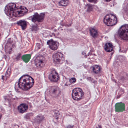
\includegraphics[width=\linewidth]{assets/images/for_presentation/exp1-2-gt.png}
    \caption{Image 2 ground truth}
  \end{subfigure}\hfill
  \begin{subfigure}[b]{0.32\textwidth}
    \centering
    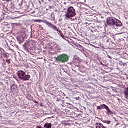
\includegraphics[width=\linewidth]{assets/images/for_presentation/exp1-3-gt.png}
    \caption{Image 3 ground truth}
  \end{subfigure}
  \caption{Visual evaluation of model trained on the TNBC dataset. Predicted lymphocytes (cyan) and ground truth lymphocytes (green).}
  \label{fig:exp1-results}
\end{figure}

\subsection{Experiment 2 - Pseudo-mask Generating Strategies}
\label{sub:exp-2}
In the second experiment, we used the 24 different pseudo-masks to train 24 different models. We wanted to compare the different models based on the pseudo-mask sets they were trained on.

\paragraph{Data}
As training data, we used the TIGER image patches. Together, 19,386 image patches were used in the training set. Pseudo-mask sets were used as ground truth labels for the training of the segmentation model. We explain the generation of these sets in detail in Section \ref{section:mask-generation}. Since these image patches come with weak annotations, we needed to evaluate the model on the TNBC dataset. For the evaluation, we used all 200 patches present in the TNBC datasets. The Dice coefficient and IoU were used as the evaluation metrics.

\paragraph{Results}
We summarized all results from this experiment in the Table \ref{tab:gen-res}. We can see that when compared to the first experiment, where we trained the same model only on the small fully annotated TNBC dataset, both the Dice coefficient and IoU improved significantly. We can also see in Figure \ref{fig:exp2-loss} that the model was able to learn better and converge faster (14 epochs on average - more than 2 times faster than the model trained solely on the TNBC dataset)

From the results, we can see that the highest Dice coefficient (52.57\%) and IoU (36.01\%) were achieved by the model that was trained on the mask set, which was created from the histogram-equalized hematoxylin image source, where the blur was not applied and where the Otsu thresholding was used. 



Next, we noticed that the histogram equalization (HE) boosts the model's performance. It consistently improved segmentation metrics across all image sources, except the ones that were using the normalized image. For example, a histogram-equalized and normalized image source with blur and adaptive thresholding reached 51.09\% Dice and 34.83\% IoU - over 11.5\% improvement in Dice coefficient and over 8\% improvement in IoU over the same non-equalized normalized pipeline (39.57\% Dice, 26.78\% IoU).

We also observed that pseudo-mask sets that used median blur were greatly outperformed by the ones that did not use it. This might be because the blur reduces noise on one hand, but on the other hand, it could distort cell boundaries and 'blend' the cell nuclei with its surroundings.

Overall, there was no universally dominant strategy - when deciding whether to use only one image source, or only blur/no-blur, or a single thresholding technique, we always observed that a different strategy could overrule it. This could also be demonstrated by the following examples:

\begin{itemize}
    \item On raw images, the best result is with no blur + Otsu thresholding (49.94\% Dice), but on normalized HE images, the best is no blur + adaptive thresholding (51.09\% Dice), and on hematoxylin HE, the top is no blur + Otsu thresholding (52.57\% Dice).
    \item In the raw setting, disabling blur (49.94\% Dice) beats enabling it (46.92\% Dice) for Otsu thresholding, but in the hematoxylin case, enabling blur (50.39\%) actually outperforms no-blur for Otsu thresholding when equalization is applied.
    \item For raw HE images with blur applied, adaptive thresholding (47.50\% Dice) beats Otsu thresholding (44.86\% Dice), whereas for normalized images with blur applied, Otsu thresholding (49.45\% Dice) outperforms adaptive thresholding (39.57\% Dice) without equalization.
\end{itemize}

These observations inspired us to design another generation of sets of pseudo-masks, where we fuse the original 24 masks into one - we explain the process of pseudo-masks fusion in Section \ref{section:mask-fusion} and the experiment itself in Subsection \ref{sub:exp-3}.

On the qualitative side, we can see in Figure \ref{fig:exp2-results} that the best model, trained on the hematoxylin image with HE, without blur and with Otsu thresholding, was able to segment cell nuclei much better than the model trained only on the small TNBC dataset. The issue here is that, although it can successfully determine whether a pixel belongs to nuclei or tissue, it cannot determine very well if the pixel should belong to the lymphocyte nuclei or some other cell type.

\begin{table}[H]
  \centering
  \begin{tabular}{ l | c | c | c | c } 
    \hline
    \textbf{Image Source\tablefootnote{HE: histogram-equalized}}    & \textbf{Blurred}  & \textbf{Threshold Type} & \textbf{Dice (\%)} & \textbf{IoU (\%)} \\
    \hline
    raw           & yes & adaptive & 44.18 & 29.28 \\
    raw           & no  & adaptive & 46.53 & 31.45 \\
    raw           & yes & otsu     & 46.92 & 31.60 \\
    raw           & no  & otsu     & \textbf{49.94} & \textbf{33.77} \\
    raw HE        & yes & otsu     & 44.86 & 29.42 \\
    raw HE        & no  & otsu     & 47.28 & 31.91 \\
    raw HE        & yes & adaptive & 47.50 & 31.98 \\
    raw HE        & no  & adaptive & 49.30 & 33.33 \\[0.5ex]
    \hline
    normalized    & yes & adaptive & 39.57 & 26.78 \\
    normalized    & no  & otsu     & 46.33 & 31.24 \\
    normalized    & no  & adaptive & 48.30 & 32.48 \\
    normalized    & yes & otsu     & 49.45 & 33.35 \\
    normalized HE & no  & otsu     & 38.30 & 25.96 \\
    normalized HE & no  & adaptive & 47.70 & 32.05 \\
    normalized HE & yes & otsu     & 48.66 & 32.66 \\
    normalized HE & yes & adaptive & \textbf{51.09} & \textbf{34.83} \\[0.5ex]
    \hline
    hematoxylin   & no  & otsu     & 41.61 & 27.46 \\
    hematoxylin   & no  & adaptive & 45.18 & 29.77 \\
    hematoxylin   & yes & adaptive & 47.94 & 32.16 \\
    hematoxylin   & yes & otsu     & 49.19 & 33.10 \\
    hematoxylin HE& yes & adaptive & 48.06 & 32.20 \\
    hematoxylin HE& yes & otsu     & 50.39 & 34.22 \\
    hematoxylin HE& no  & adaptive & 52.35 & 35.97 \\
    hematoxylin HE& no  & otsu     & \textbf{52.57} & \textbf{36.01} \\
    \hline
  \end{tabular}
  \caption{Dice and IoU percentages for the models trained on different pseudo‐mask generation strategies.}
  \label{tab:gen-res}
\end{table}

\begin{figure}[H]
\begin{centering}
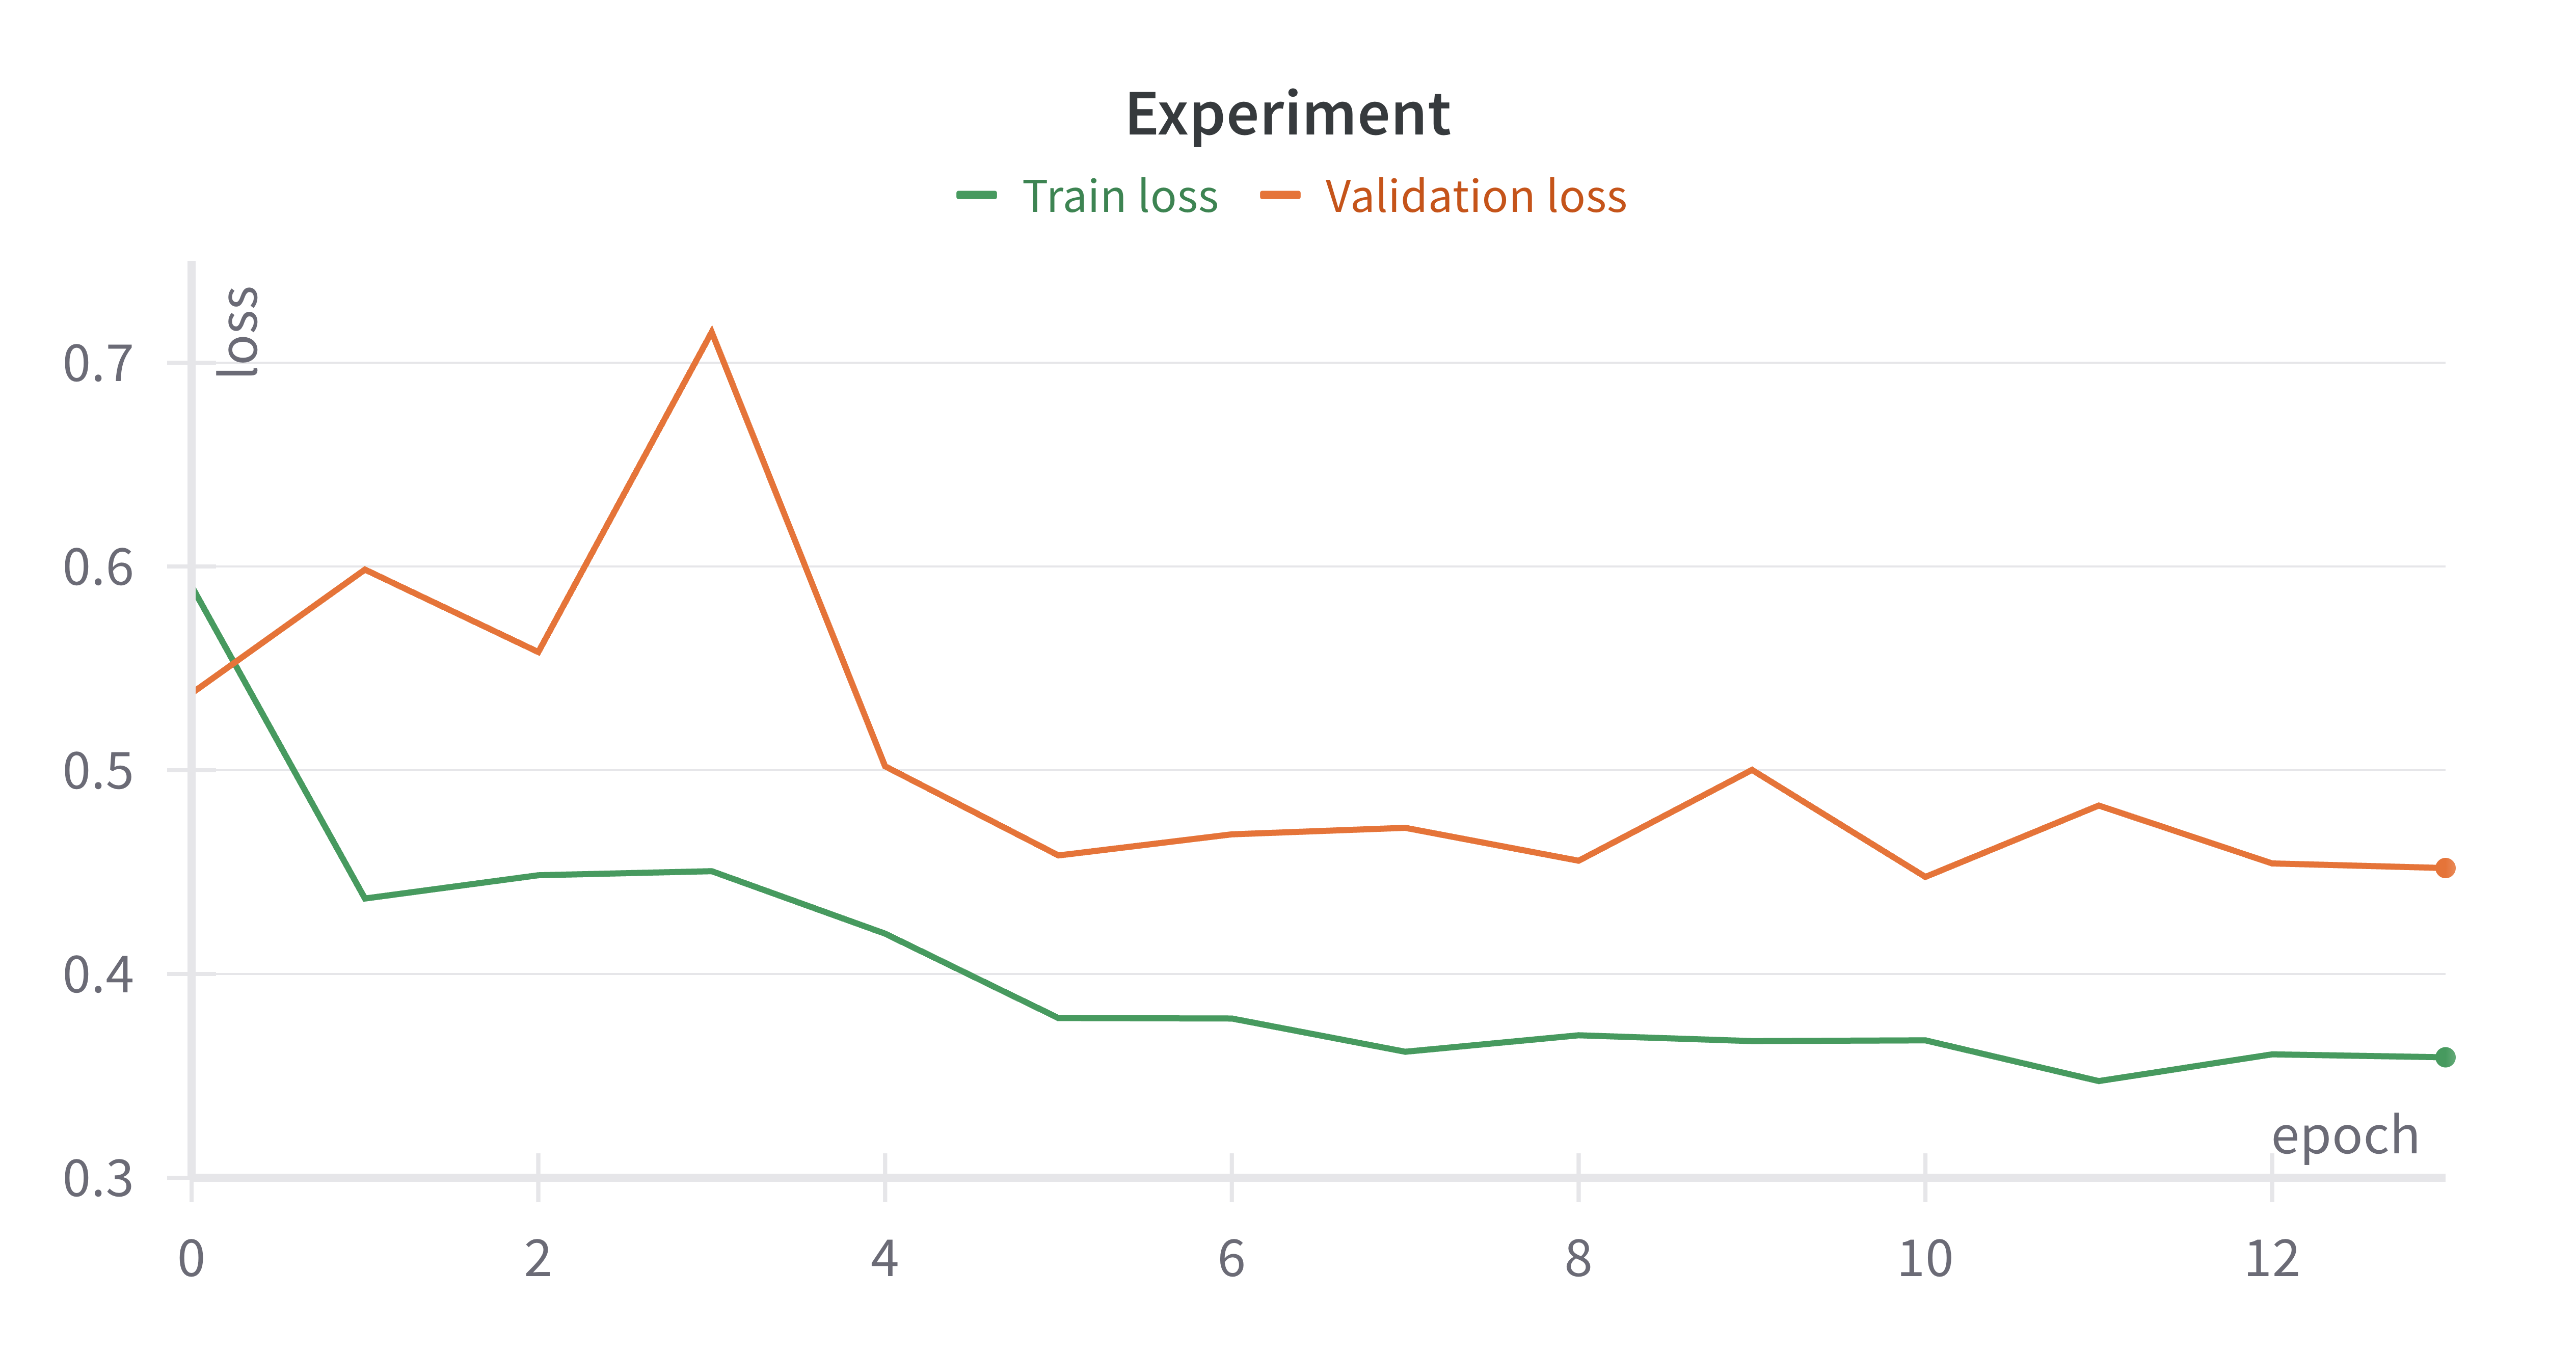
\includegraphics[width=\textwidth]{assets/images/for_presentation/exp2-loss.png}
\par\end{centering}
\caption{The loss function during training (green) and validation (orange) of the best model trained with the hematoxylin histogram-equalized pseudo-mask, created without blur applied and with Otsu thresholding.
\label{fig:exp2-loss}}
\end{figure}

\begin{figure}[H]
  \centering
  % First row of three subfigures
  \begin{subfigure}[b]{0.32\textwidth}
    \centering
    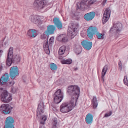
\includegraphics[width=\linewidth]{assets/images/for_presentation/exp2-1-pred.png}
    \caption{Image 1 prediction}
  \end{subfigure}\hfill
  \begin{subfigure}[b]{0.32\textwidth}
    \centering
    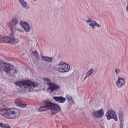
\includegraphics[width=\linewidth]{assets/images/for_presentation/exp-2-2-pred.png}
    \caption{Image 2 prediction}
  \end{subfigure}\hfill
  \begin{subfigure}[b]{0.32\textwidth}
    \centering
    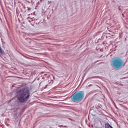
\includegraphics[width=\linewidth]{assets/images/for_presentation/exp2-3-pred.png}
    \caption{Image 3 prediction}
  \end{subfigure}

  % Line break to start the second row; adjust vertical space as needed
  \par\vspace{0.5em}

  % Second row of three subfigures
  \begin{subfigure}[b]{0.32\textwidth}
    \centering
    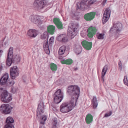
\includegraphics[width=\linewidth]{assets/images/for_presentation/exp2-2-gt.png}
    \caption{Image 1 ground truth}
  \end{subfigure}\hfill
  \begin{subfigure}[b]{0.32\textwidth}
    \centering
    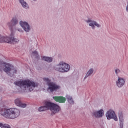
\includegraphics[width=\linewidth]{assets/images/for_presentation/exp2-1-gt.png}
    \caption{Image 2 ground truth}
  \end{subfigure}\hfill
  \begin{subfigure}[b]{0.32\textwidth}
    \centering
    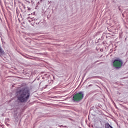
\includegraphics[width=\linewidth]{assets/images/for_presentation/exp2-3-gt.png}
    \caption{Image 3 ground truth}
  \end{subfigure}
  \caption{Visual evaluation of the best model trained with the hematoxylin HE pseudo-mask, created without blur applied and with Otsu thresholding. Predicted lymphocytes (cyan) and ground truth lymphocytes (green).}
  \label{fig:exp2-results}
\end{figure}

\subsection{Experiment 3 - Pseudo-mask Fusing Strategies}
\label{sub:exp-3}
The third experiment expanded further on the idea that different pseudo-mask sets can sometimes better capture the nuclei under varying conditions, as we saw in experiment 2 in Subsection \ref{sub:exp-2}. For this purpose, we try to combine the power of different pseudo-mask sets to create one pseudo-mask that will be used for the training. In this experiment, we want to compare different fusing strategies for the resulting pseudo-mask.

\paragraph{Data}
Similarly to Experiment 2, we work with the TIGER dataset as the training set for the model, and evaluate it on the TNBC dataset. The major change is the usage of fused masks. We present the different fusing strategies in Section \ref{section:mask-fusion}. Together, there are 8 fused pseudo-mask sets, created with both best quartile agreement levels and voting consensus. The rest of the experiment setting is the same as it was in Experiment 2.

\paragraph{Results}
From the results summary presented in Table \ref{tab:fusion-strategies}, we can clearly state that the consensus method - where either 24 out of 24, 23 out of 24, 22 out of 24, or 21 out of 24 masks voted for a pixel in a fused pseudo-mask - heavily outperformed the quartile agreement strategy, where the best 100\%, 75\%, 50\%, or 25\% of the pseudo-masks voted for a pixel (if at least one mask voted for the pixel, the pixel was set as foreground - nuclei). The order of the best pseudo-masks was determined by the previous experiment, which we describe in Subsection \ref{sub:exp-2}, specifically the Dice coefficient values.

The best model trained on the consensus strategy achieved a Dice coefficient of 53.53\%, while the best model trained on the quartile strategy achieved a Dice of 42.93\%, by 10.6\% worse than the best consensus strategy model.

We also compare these two best models in terms of train and validation loss, which we can see in the Figure \ref{fig:exp3-loss}. There, we see that the consensus model was able to learn better during training as well. The quartile model was not able to learn that good, and the training even stopped earlier.

Finally, we compare these two models visually, in the Figure \ref{fig:exp3-results}. From the figure, it is clear that the quartile model also captures cell nuclei surroundings, and is more prone to mark non-lymphocyte nuclei as lymphocyte nuclei. The consensus model is much better at segmenting only the cell nuclei, however, the same issue as in experiment 2 prevails - the model can identify cell nuclei, but it is harder for it to tell if it is a lymphocyte or non-lymphocyte nucleus.

When we compare the best model from this experiment - the consensus model (53.53\% Dice) with the best model from experiment 2 - the model trained on the HE hematoxylin image, without blur and Otsu thresholding (52.57\%), we see that by fusing the masks and selecting the correct fusion strategy, we were able to improve the model's performance by 0.96\%.

\begin{table}[H]
  \centering
  \begin{tabular}{ l | l | c | c } 
    \hline
    \textbf{Masks Set Type} & \textbf{Mask Set} & \textbf{Dice (\%)} & \textbf{IoU (\%)} \\
    \hline
      consensus & leave 0 out & 50.88 & 34.96 \\
      consensus & leave 1 out & \textbf{53.53} & \textbf{37.42} \\
      consensus & leave 2 out & 52.31 & 36.35 \\
      consensus & leave 3 out & 52.58 & 36.33 \\
    \hline
      quartile  & top 100\%   & 41.11 & 26.40 \\
      quartile  & top 75\%    & 40.35 & 25.72 \\
      quartile  & top 50\%    & \textbf{42.93} & \textbf{27.89} \\
      quartile  & top 25\%    & 42.59 & 27.61 \\
    \hline
  \end{tabular}
  \caption{Dice and IoU percentages for the models trained on different pseudo‐mask fusion strategies.}
  \label{tab:fusion-strategies}
\end{table}

\begin{figure}[H]
\begin{centering}
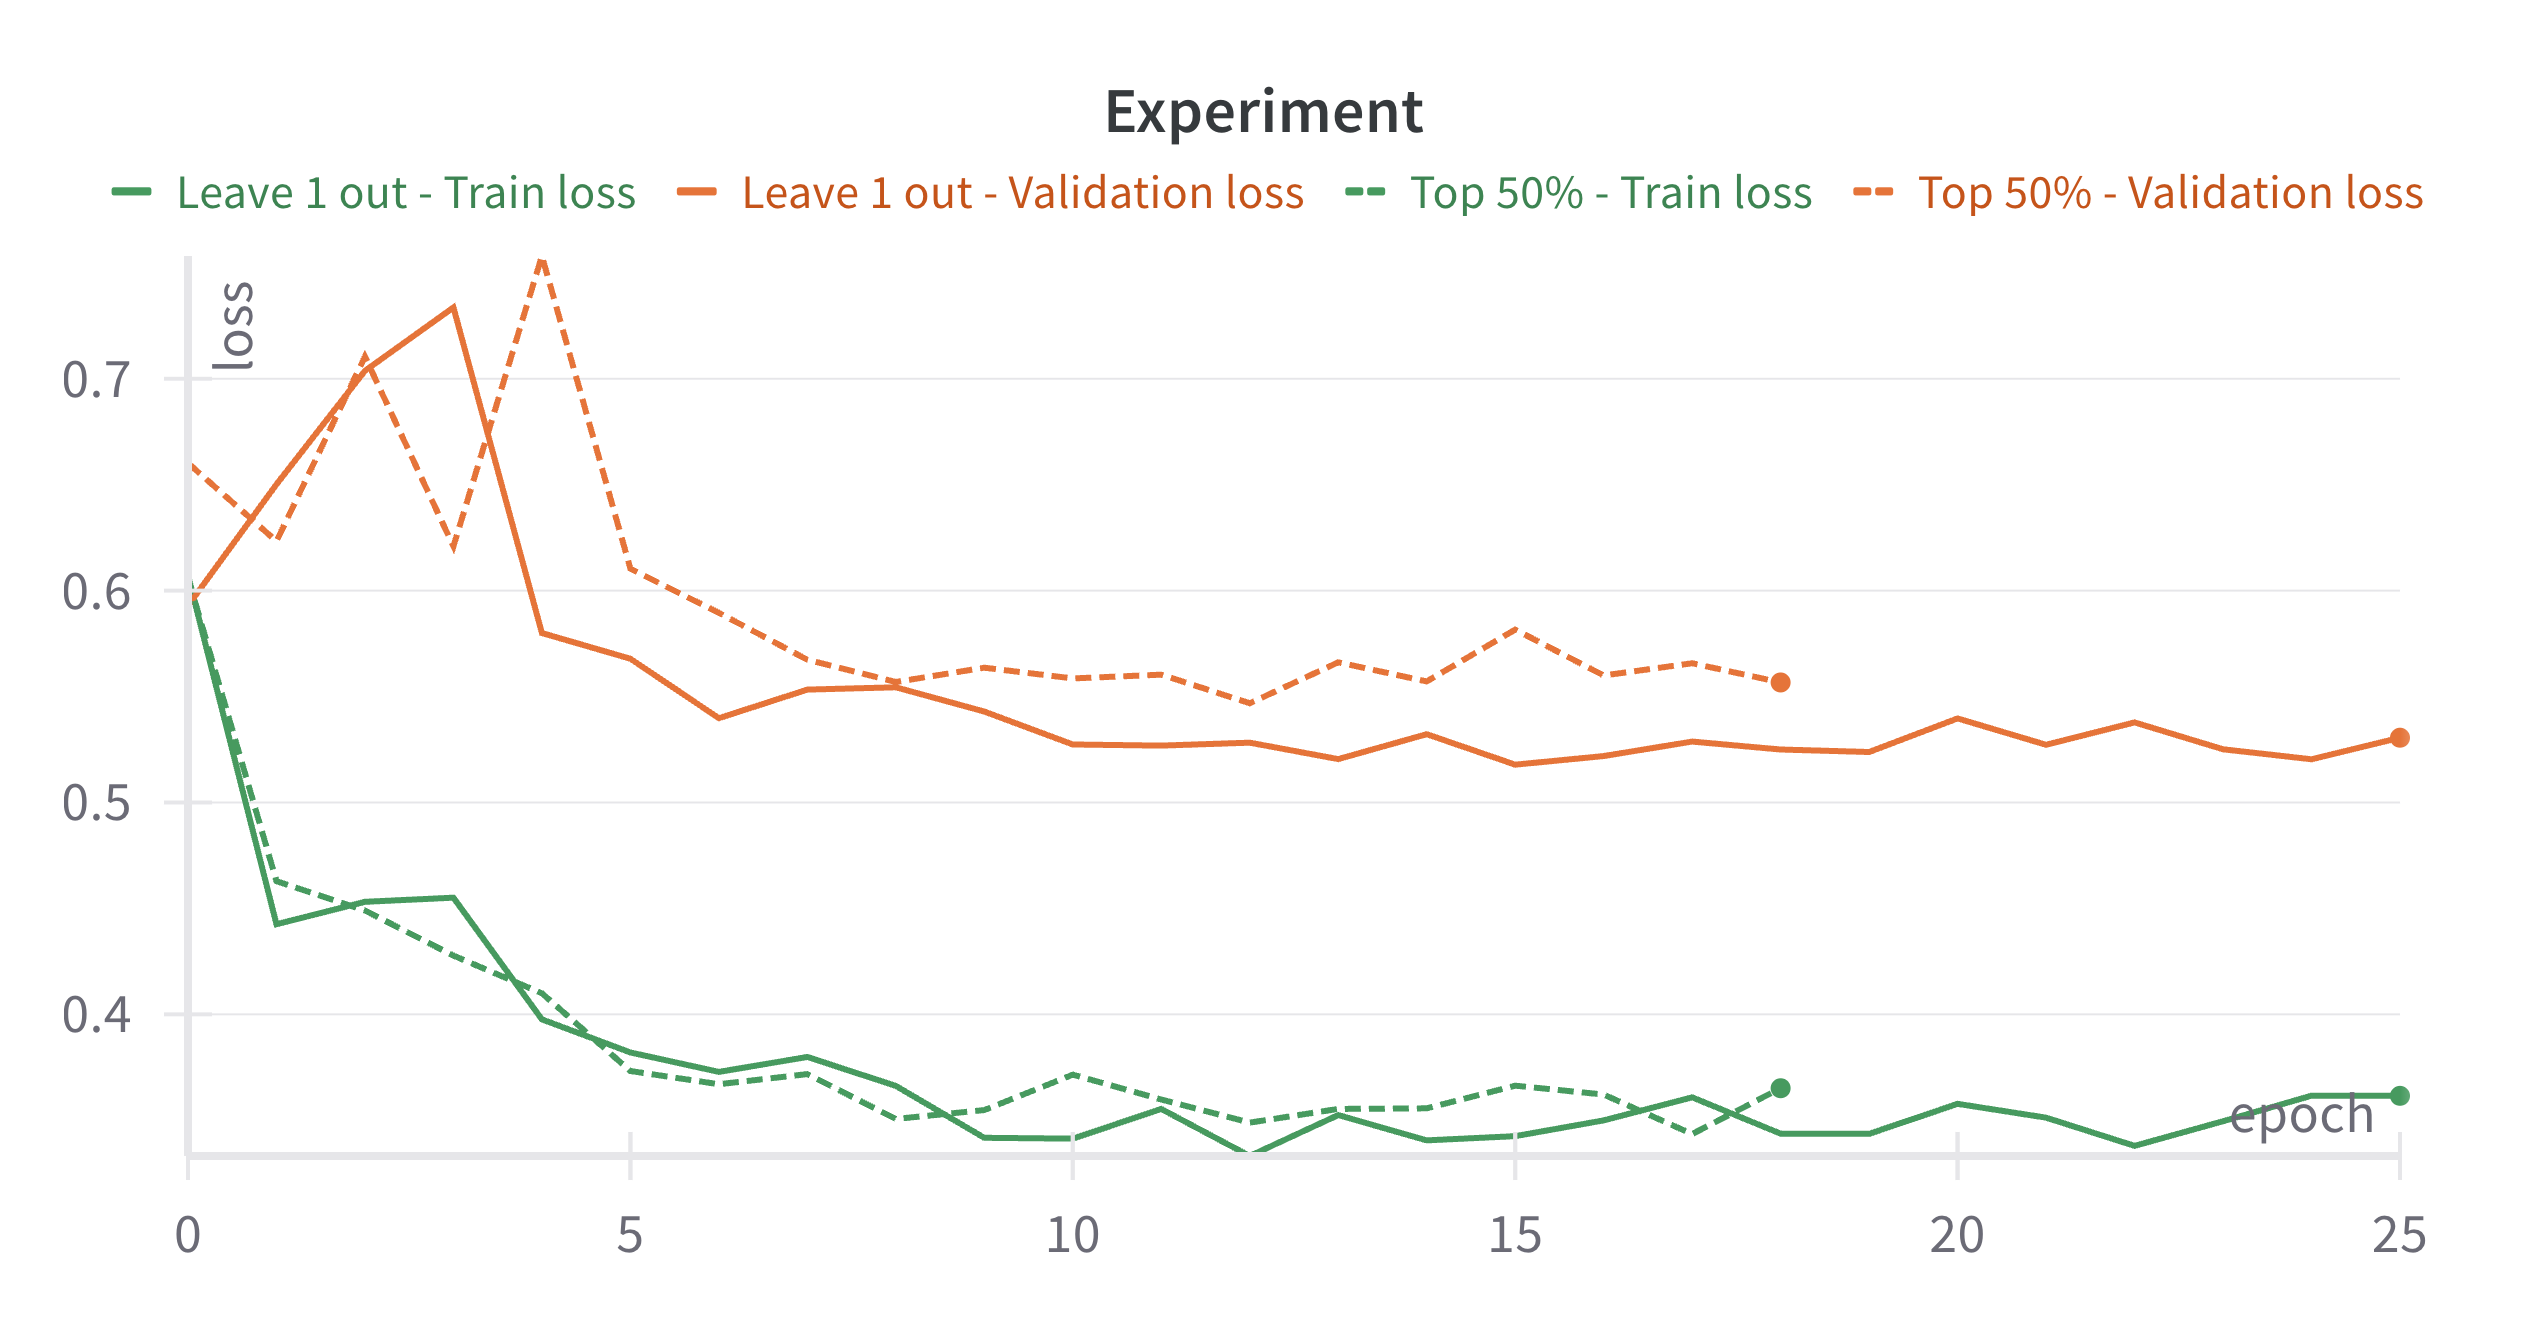
\includegraphics[width=\textwidth]{assets/images/for_presentation/exp3-loss.png}
\par\end{centering}
\caption{The loss function during training (green dashed) and validation (orange dashed) of the best model trained with the quartile strategy of fusing pseudo-masks, and the loss function during training (green solid) and validation (orange solid) of the best model trained with the consensus strategy of fusing pseudo-masks.
\label{fig:exp3-loss}}
\end{figure}

\begin{figure}[H]
  \centering
  % First row of three subfigures
  \begin{subfigure}[b]{0.32\textwidth}
    \centering
    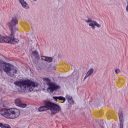
\includegraphics[width=\linewidth]{assets/images/for_presentation/exp3-1-pred-top50.png}
    \caption{Image 1 prediction - Top 50\%}
  \end{subfigure}\hfill
  \begin{subfigure}[b]{0.32\textwidth}
    \centering
    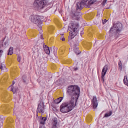
\includegraphics[width=\linewidth]{assets/images/for_presentation/exp3-2-pred-top50.png}
    \caption{Image 2 prediction - Top 50\%}
  \end{subfigure}\hfill
  \begin{subfigure}[b]{0.32\textwidth}
    \centering
    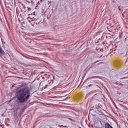
\includegraphics[width=\linewidth]{assets/images/for_presentation/exp3-3-pred-top50.png}
    \caption{Image 3 prediction - Top 50\%}
  \end{subfigure}

  % Line break to start the second row; adjust vertical space as needed
  \par\vspace{0.5em}
  
 % Second row of three subfigures
   \begin{subfigure}[b]{0.32\textwidth}
    \centering
    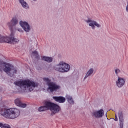
\includegraphics[width=\linewidth]{assets/images/for_presentation/exp3-1-pred-l1o.png}
    \caption{Image 1 prediction - Leave 1 out}
  \end{subfigure}\hfill
  \begin{subfigure}[b]{0.32\textwidth}
    \centering
    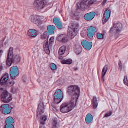
\includegraphics[width=\linewidth]{assets/images/for_presentation/exp3-2-pred-l1o.png}
    \caption{Image 2 prediction - Leave 1 out}
  \end{subfigure}\hfill
  \begin{subfigure}[b]{0.32\textwidth}
    \centering
    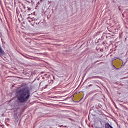
\includegraphics[width=\linewidth]{assets/images/for_presentation/exp3-3-pred-l1o.png}
    \caption{Image 3 prediction - Leave 1 out}
  \end{subfigure}

  % Line break to start the second row; adjust vertical space as needed
  \par\vspace{0.5em}

  % Third row of three subfigures
  \begin{subfigure}[b]{0.32\textwidth}
    \centering
    \includegraphics[width=\linewidth]{assets/images/for_presentation/exp3-1-gt.png}
    \caption{Image 1 ground truth}
  \end{subfigure}\hfill
  \begin{subfigure}[b]{0.32\textwidth}
    \centering
    \includegraphics[width=\linewidth]{assets/images/for_presentation/exp3-2-gt.png}
    \caption{Image 2 ground truth}
  \end{subfigure}\hfill
  \begin{subfigure}[b]{0.32\textwidth}
    \centering
    \includegraphics[width=\linewidth]{assets/images/for_presentation/exp3-3-gt.png}
    \caption{Image 3 ground truth}
  \end{subfigure}
  \caption{Visual comparison of the best models trained with the quartile (top row) and consensus strategies (middle row), and ground truth (bottom row). Predicted lymphocytes (cyan) and ground truth lymphocytes (green).}
  \label{fig:exp3-results}
\end{figure}


\subsection{Experiment 4 - Transfer Learning}
In the last experiment, we wanted to build on the results of experiment 3. We decided to take the best model from that experiment and fine-tune it using a portion of data from the fully annotated TNBC dataset. We also experimented with the encoder freezing during the training to see if we could further improve the model's performance. 

\paragraph{Data}
We use the model pretrained on the TIGER dataset. For the fine-tuning, we use the TNBC dataset, with the exact same 3-fold split as we used in experiment 1, which we describe in Subsection \ref{sub:exp-1}. We always used 2 folds for fine-tuning and 1 fold for evaluation of the model. The final evaluation metrics were computed as a weighted average of the metrics reported in each fold evaluation. We fine-tuned the model under two conditions. We tried fine-tuning it with a frozen encoder, which means that the weights of the encoder were not updated during the training, only the weights of the decoder. In the second approach, we trained the whole model, both the encoder and the decoder.

\paragraph{Results}
In the Table \ref{tab:transfer}, we have summarized the final evaluation metrics of this experiment. We can see that when compared to the best model from experiment 3 (53.53\% Dice) - the consensus model, where 23 out of 24 masks voted for a pixel - both the model with unfrozen encoder (55.01\% Dice) and the one with frozen encoder (57.59\% Dice) were able to slightly improve. Overall, the best model was the model with frozen encoder during the fine-tuning - it achieved a Dice coefficient of 57.59\% and IoU of 41.25\%.

On the graph showing the training and validation loss of the model with frozen encoder in Figure \ref{fig:exp4-loss} we can see that the fine-tuning enabled the model to learn slightly more, but also that the training was very short (13 epochs) since the model could not improve further on the validation loss.

Finally, in Figure \ref{fig:exp4-results} we observe a similar behavior to the best models from experiments 2 and 3 - that the model can recognize the cell nuclei pixels, but has a problem of differentiating between the pixels that belong to lymphocyte nuclei and non-lymphocyte nuclei.

\begin{table}[H]
  \centering
  \begin{tabular}{ p{5cm} | p{3cm} | p{3cm} } 
    \hline
    \textbf{Encoder status} & \textbf{Dice (\%)} & \textbf{IoU (\%)} \\
    \hline
      Unfrozen & 55.01 & 38.6 \\
      Frozen   & \textbf{57.59} & \textbf{41.25} \\
    \hline
  \end{tabular}
  \caption{Dice and IoU percentages for the models fine-tuned on the TNBC dataset.}
  \label{tab:transfer}
\end{table}

\begin{figure}[H]
\begin{centering}
\includegraphics[width=\textwidth]{assets/images/for_presentation/exp4-loss.png}
\par\end{centering}
\caption{The loss function during training (green) and validation (orange) of the model fine-tuned with the frozen encoder.
\label{fig:exp4-loss}}
\end{figure}

\begin{figure}[H]
  \centering
  % First row of three subfigures
  \begin{subfigure}[b]{0.32\textwidth}
    \centering
    \includegraphics[width=\linewidth]{assets/images/for_presentation/exp4-1-pred.png}
    \caption{Image 1 prediction}
  \end{subfigure}\hfill
  \begin{subfigure}[b]{0.32\textwidth}
    \centering
    \includegraphics[width=\linewidth]{assets/images/for_presentation/exp4-2-pred.png}
    \caption{Image 2 prediction}
  \end{subfigure}\hfill
  \begin{subfigure}[b]{0.32\textwidth}
    \centering
    \includegraphics[width=\linewidth]{assets/images/for_presentation/exp4-3-pred.png}
    \caption{Image 3 prediction}
  \end{subfigure}

  % Line break to start the second row; adjust vertical space as needed
  \par\vspace{0.5em}

  % Second row of three subfigures
  \begin{subfigure}[b]{0.32\textwidth}
    \centering
    \includegraphics[width=\linewidth]{assets/images/for_presentation/exp4-1-gt.png}
    \caption{Image 1 ground truth}
  \end{subfigure}\hfill
  \begin{subfigure}[b]{0.32\textwidth}
    \centering
    \includegraphics[width=\linewidth]{assets/images/for_presentation/exp4-2-gt.png}
    \caption{Image 2 ground truth}
  \end{subfigure}\hfill
  \begin{subfigure}[b]{0.32\textwidth}
    \centering
    \includegraphics[width=\linewidth]{assets/images/for_presentation/exp4-3-gt.png}
    \caption{Image 3 ground truth}
  \end{subfigure}
  \caption{Visual evaluation of the model fine-tuned with the frozen encoder. Predicted lymphocytes (cyan) and ground truth lymphocytes (green).}
  \label{fig:exp4-results}
\end{figure}

\subsection{Experiments Summary}
To summarize the experiments, we decided to put the evaluation metrics of the best model from each experiment into a single Table \ref{tab:summary-experiments}. There, we can see that in each subsequent experiment, we were able to improve the overall performance of the corresponding model. The best model overall is the one trained on the TIGER dataset and the consensus fusion strategy, where 23 out of 24 masks voted for a pixel to be foreground (lymphocyte nuclei) and then fine-tuned on the TNBC dataset, with the encoder frozen during the training.

\begin{table}[H]
  \centering
  \begin{tabular}{ l | c | c } 
    \hline
    \textbf{Experiment}                                  & \textbf{Best Dice (\%)} & \textbf{Best IoU (\%)} \\
    \hline
    1 – Training with full annotations                   & 18.91                   & 10.64                  \\
    2 – Mask generating strategies                       & 52.57                   & 36.01                  \\
    3 – Mask fusing strategies                           & 53.53                   & 37.42                  \\
    4 – Transfer Learning                                & \textbf{57.59}          & \textbf{41.45}          \\
    \hline
  \end{tabular}
  \caption{Comparison of best Dice and IoU across experiments.}
  \label{tab:summary-experiments}
\end{table}


\section{Tools}
The whole project was written in the Python programming language version 3.12  \cite{python}. We used Python libraries such as NumPy \cite{numpy} for efficient numerical operations, and Matplotlib \cite{matplotlib} for the image, masks, and overlay visualizations. Furthermore, we utilized the power of Jupyter Notebooks \cite{jupyter} to be able to run parts of code and easily explore the data during the preprocessing and pseudo-mask creation stages, and also to be able to upload data and submit training on the remote clusters.

For the image manipulation, transformation, and other computer vision operations during the preprocessing, pseudo-masks generation, and pseudo-masks fusion stages, we relied on the OpenCV Python library \cite{open-cv}. For the multi-target Macenko stain normalization, we used the existing implementation from \cite{torchstain}. The whole preprocessing and pseudo-masks creation process was executed locally on a MacBook Air with an M1 Silicon chip, with 16 GB of RAM.

Libraries and frameworks such as scikit-learn \cite{scikit-learn}, PyTorch \cite{pytorch}, PyTorch Lightning \cite{pytorch-ligthning}, and Segmentation Models PyTorch \cite{smp} were used for implementation of the classical machine learning baselines as well as for building the deep learning segmentation model to reduce the boilerplate code and make use of trusted and validated approaches implemented in those modules.

For the development and debugging, we used the PyCharm \cite{pycharm} integrated development environment. We also used Git \cite{git} for version management and GitHub \cite{github} for remote control of our project.

The training of all models was done remotely in the cloud environment, since this was the fastest and most feasible option. We utilized the Azure Machine Learning Studio \cite{azure-ml} for this purpose. As a compute device, we used the virtual machine, which provides 24 CPU cores, 448 GB of RAM, a 2.9 TB disk, and 4 NVIDIA Tesla V100 GPUs. The computationally expensive tasks used CUDA \cite{cuda} for GPU acceleration, so that the training could be completed in a shorter amount of time compared to the CPU. For easier monitoring, logging, data visualization, and the overall improved management of the whole training process and evaluation process, we used the Weights and Biases \cite{wandb}, where we could save, compare, and plot different trainings and runs.